\documentclass[12pt, a4paper]{article}

% --- Packages ---
\usepackage[utf8]{inputenc}
\usepackage{mathptmx}
\usepackage[left=0.9in,right=0.9in,top=0.9in,bottom=0.9in]{geometry}
\usepackage{graphicx}
\usepackage{xcolor}
\usepackage{fancyhdr}
\usepackage{titlesec}
\usepackage{array}
\usepackage{tabularx}
\usepackage{setspace}
\usepackage{float}
\usepackage{enumitem}
\usepackage{booktabs}
\usepackage{longtable}
\usepackage{caption}
\usepackage{subcaption}
\usepackage{amsmath}
\usepackage{listings}
\usepackage[hidelinks,plainpages=false,pdfpagelabels,hypertexnames=false]{hyperref}
\usepackage{tikz}
\usepackage{eso-pic}
\usepackage{pgfplots}
\pgfplotsset{compat=1.18}
\usetikzlibrary{arrows.meta, positioning, shapes.geometric, calc, shapes.multipart, fit, backgrounds}

% --- Custom formatting ---
\setstretch{1.5}
\setlength{\headheight}{15pt}
\setlength{\parindent}{0pt}
\setlength{\parskip}{4pt}
\setlist[itemize]{leftmargin=1.8em, itemsep=3pt, topsep=5pt, parsep=0pt, partopsep=0pt}
\setlist[itemize,2]{leftmargin=1.5em, itemsep=2pt, topsep=3pt}
\setlist[enumerate]{leftmargin=1.8em, itemsep=3pt, topsep=5pt, parsep=0pt, partopsep=0pt}
\setlist[enumerate,2]{leftmargin=1.5em, itemsep=2pt, topsep=3pt}

% Custom colors
\definecolor{phgreen}{RGB}{169, 209, 142}
\definecolor{blockbg}{RGB}{245, 245, 245}
\definecolor{primaryblue}{RGB}{41, 128, 185}
\definecolor{secondarygreen}{RGB}{39, 174, 96}
\definecolor{warnorange}{RGB}{230, 126, 34}

% Code listing style
\lstset{
	basicstyle=\ttfamily\small,
	breaklines=true,
	frame=single,
	numbers=left,
	numberstyle=\tiny,
	tabsize=2,
	backgroundcolor=\color{blockbg}
}

% Section headings
\titleformat{\section}[block]{\normalfont\bfseries\fontsize{16pt}{18pt}\selectfont\filcenter}{\thesection.}{0.5em}{}
\titleformat{\subsection}[hang]{\normalfont\bfseries\fontsize{14pt}{16pt}\selectfont}{\thesubsection}{0.5em}{}
\titleformat{\subsubsection}[hang]{\normalfont\bfseries\fontsize{14pt}{16pt}\selectfont}{\thesubsubsection}{0.5em}{}

% Section spacing
\titlespacing*{\section}{0pt}{18pt plus 4pt minus 2pt}{10pt plus 2pt minus 2pt}
\titlespacing*{\subsection}{0pt}{14pt plus 3pt minus 2pt}{8pt plus 2pt minus 2pt}
\captionsetup[figure]{name=Figure}
\numberwithin{figure}{section}
\numberwithin{table}{section}

% Header and Footer styles
\setlength{\headsep}{10pt}
\setlength{\footskip}{26pt}

\fancypagestyle{frontstyle}{
	\fancyhf{}
	\fancyfoot[C]{\thepage}
	\renewcommand{\headrulewidth}{0pt}
	\renewcommand{\footrulewidth}{0pt}
}

\fancypagestyle{mainstyle}{
	\fancyhf{}
	\fancyhead[R]{\small\itshape Smart Energy Meter}
	\fancyfoot[C]{\thepage}
	\renewcommand{\headrulewidth}{0pt}
	\renewcommand{\footrulewidth}{0pt}
}

\fancypagestyle{plain}{
	\fancyhf{}
	\fancyhead[R]{\small\itshape Smart Energy Meter}
	\fancyfoot[C]{\thepage}
	\renewcommand{\headrulewidth}{0pt}
	\renewcommand{\footrulewidth}{0pt}
}

\pagestyle{frontstyle}

% Border helper for front pages only
\newlength{\pageframeinset}
\newlength{\leftframeinset}
\setlength{\pageframeinset}{0.50in}
\setlength{\leftframeinset}{0.50in}
\newcommand{\drawfrontborder}{
	\begin{tikzpicture}[remember picture, overlay]
		\draw[line width=0.8pt]
		([xshift=\leftframeinset,yshift=-\pageframeinset]current page.north west) rectangle
		([xshift=-\pageframeinset,yshift=\pageframeinset]current page.south east);
	\end{tikzpicture}
}

\begin{document}
	
	% ==========================================
	% PAGE 1: TITLE PAGE
	% ==========================================
	\thispagestyle{empty}
	\begin{center}
		\vspace*{0.35cm}
		{\Large \textbf{A Mini Project Report}}\\[0.25cm]
		{\Large \textbf{On}}\\[0.25cm]
		{\Large \textbf{``Smart Energy Meter''}}\\[0.7cm]
		
		Submitted to Savitribai Phule Pune University, Pune, as a part of the academic mini project\\
		requirements for the completion of\\[0.65cm]
		
		{\Large \textbf{Bachelor of Technology}}\\[0.2cm]
		{\Large \textbf{in}}\\[0.2cm]
		{\Large \textbf{Information Technology}}\\[0.65cm]
		
		Submitted by :-\\[0.2cm]
		TY-B\\[0.2cm]
		\begin{tabular}{ll}
			Raman Bhise & Roll No.: B52 \\
			Panchakshari Chakor & Roll No.: B53 \\
			Rutika Parekar & Roll No.: B60 \\
			Omkar Jagtap & Roll No.: B65 \\
		\end{tabular}\\[0.5cm]
		
		
\includegraphics[width=0.21\textwidth]{ghrcem.png}\\[0.55cm]
		
		{\Large \textbf{Department of Information Technology}}\\[0.2cm]
		{\Large \textbf{G H Raisoni College of Engineering and Management, Pune}}\\
		(An Empowered Autonomous Institute Affiliated to SPPU, Pune)\\[0.45cm]
		{\Large \textbf{Academic Year 2025-26}}\\
		{\Large \textbf{Semester-VI}}
	\end{center}
	\drawfrontborder
	\newpage
	\pagenumbering{roman}
	\setcounter{page}{1}
	
	% ==========================================
	% PAGE 2: CERTIFICATE
	% ==========================================
	\thispagestyle{frontstyle}
	\begin{center}
		
\includegraphics[width=0.8\textwidth]{Picture2.png}
		\vspace{0.3cm}
		
		{\Large \textbf{CERTIFICATE}}\\[0.8cm]
	\end{center}
	
	\begin{center}
		This is to certify that the mini project titled
	\end{center}
	
	\begin{center}
		\makebox[0.8\textwidth]{\Large \textbf{Smart Energy Meter}}\\[0.4cm]
	\end{center}
	
	\begin{center}
		embodies the original work carried out by:
	\end{center}
	
	\begin{center}
		
		\begin{tabular}{ll}
			\textbf{Raman Bhise} & \textbf{Roll No.: B52} \\
			\textbf{Panchakshari Chakor} & \textbf{Roll No.: B53} \\
			\textbf{Rutika Parekar} & \textbf{Roll No.: B60} \\
			\textbf{Omkar Jagtap} & \textbf{Roll No.: B65} \\
		\end{tabular}
		
	\end{center}
	
	\vspace{0.2cm}
	\noindent This mini project submission is made as a partial fulfillment of the requirements for the B. Tech. Degree, VI Semester, of Pune University during the academic year 2025 - 2026.\\[2cm]
	
	\noindent
	\begin{tabular*}{\textwidth}{@{\extracolsep{\fill}}ll}
		\textbf{Mr. Dasganu Hakke} & \textbf{Dr. Poonam Gupta} \\
		Project Guide & Head of Department \\[1.4cm]
		\rule{3.8cm}{0.4pt} & \\
		External Examiner & \\
	\end{tabular*}\\[0.5cm]
	
	\noindent \textbf{Date: \rule{2.7cm}{0.4pt}}\\[0.2cm]
	\noindent \textbf{Place: Pune}
	
	\drawfrontborder
	\newpage
	
	% ==========================================
	% PAGE 3: ACKNOWLEDGMENT
	% ==========================================
	\thispagestyle{frontstyle}
	\begin{center}
		{\Large \textbf{ACKNOWLEDGMENT}}\\[1cm]
	\end{center}
	
	\noindent We would like to express our sincere thanks to \textbf{Dr. Poonam Gupta}, Head of Information Technology Department, for continuous support \& valuable suggestions.
	
	\noindent We would like to thank \textbf{Mr. Dasganu Hakke}, for his valuable support in providing us with the required information, guidance and light of knowledge, we could complete this Microproject.
	
	\noindent We take this opportunity to thank all the staff members of the Department of Information Technology Engineering for their help whenever required.
	
	\noindent We take this opportunity to thank our Director In-Charge, \textbf{Dr. N. B. Hulle} and Campus Director, \textbf{Dr. R. D. Kharadkar}, for his whole hearted support, motivation \& valuable suggestions.
	
	\noindent Finally, we would like to give special thanks to all staff members of the Department of Information Technology, GH Raisoni College of Engineering and Management, Pune \& our friends for their kind support.\\[0.5cm]
	
	\begin{flushright}
	\begin{tabular}{ll}
		Raman Bhise & (Roll No.: B52) \\
		Panchakshari Chakor & (Roll No.: B53) \\
		Rutika Parekar & (Roll No.: B60) \\
		Omkar Jagtap & (Roll No.: B65) \\
	\end{tabular}
	\end{flushright}
	
	\drawfrontborder
	
	\newpage
	
	% ==========================================
	% PAGE 4: ABSTRACT
	% ==========================================
	\thispagestyle{frontstyle}
	\begin{center}
		{\Large \textbf{ABSTRACT}}\\[1cm]
	\end{center}
	
	This mini project presents a smart energy meter for appliance-level monitoring in homes and small labs. The work started from a simple gap in existing billing: monthly units are visible, but appliance-wise consumption is not. To build a usable prototype, the project required low-cost sensing hardware, safe AC-to-DC isolation, WiFi communication, and a dashboard that could present live readings clearly.
	
	The implemented setup uses an ESP32 DevKit V1 with ZMPT101B for voltage sensing and ACS712 for current sensing. Firmware samples AC waveforms, computes RMS and power parameters, updates the OLED display, and sends telemetry through MQTT. On the server side, a Flask backend receives the data, runs machine learning inference for prediction and anomaly checks, and streams updates to the web dashboard with relay control support.
	
	Validation was carried out with practical loads such as a 600W kettle and a 65W charger. After calibration, the system produced stable readings and stayed close to reference values, with lower error on higher loads and comparatively higher deviation at very low current levels. The final prototype delivers clear device-level visibility, remote switching, and a practical base for future expansion to multi-appliance monitoring.
	
	\drawfrontborder
	
	\newpage
	
	% ==========================================
	% PAGE 5: INDEX
	% ==========================================
	\thispagestyle{frontstyle}
	\begin{center}
		{\Large \textbf{Index}}\\[1cm]
	\end{center}
	
	\renewcommand{\arraystretch}{2} % Taller rows to match the document
	\begin{center}
		\begin{tabular}{c p{0.6\textwidth} c}
			\textbf{S N} & \textbf{Details} & \textbf{Page No.} \\
			\textbf{1} & \textbf{Introduction} & \pageref{sec:intro} \\
			\textbf{2} & \textbf{Objective of the Project} & \pageref{sec:objective} \\
			\textbf{3} & \textbf{Tools and Technologies Used} & \pageref{sec:tools} \\
			\textbf{4} & \textbf{Project Design / Methodology} & \pageref{sec:design} \\
			\textbf{5} & \textbf{Implementation / Working} & \pageref{sec:implementation} \\
			\textbf{6} & \textbf{Results / Output} & \pageref{sec:results} \\
			\textbf{7} & \textbf{Conclusion} & \pageref{sec:conclusion} \\
			\textbf{8} & \textbf{References} & \pageref{sec:references} \\
		\end{tabular}
	\end{center}
	\renewcommand{\arraystretch}{1} % Reset array stretch for rest of doc
	
	\drawfrontborder
	
	\newpage
	
	% ==========================================
	% PAGE 6: INTRODUCTION (Header/Footer start)
	% ==========================================
	% Start main content with Arabic page numbering
	\pagenumbering{arabic}
	\setcounter{page}{1}
	\pagestyle{mainstyle}
	
	\section{INTRODUCTION}\label{sec:intro}
	
	\subsection{Overview}
	
	This project is a per-appliance energy monitoring system built around the ESP32 DevKit V1 microcontroller. The device connects between a wall socket and an appliance to measure voltage, current, and power in real time. Fig.~\ref{fig:system-overview} shows the block diagram of the proposed system.
	
	\begin{figure}[H]
		\centering
		\begin{tikzpicture}[
			node distance=1.8cm,
			block/.style={rectangle, draw, fill=primaryblue!20, minimum width=2.2cm, minimum height=1cm, align=center, rounded corners=3pt},
			arrow/.style={-{Stealth[length=2.5mm]}, thick}
		]
		\node[block] (appliance) {Appliance\\(Load)};
		\node[block, right=of appliance] (meter) {Smart\\Energy Meter};
		\node[block, right=of meter] (cloud) {Backend\\Server};
		\node[block, right=of cloud] (dashboard) {Web\\Dashboard};
		\node[block, below=1cm of meter] (oled) {OLED\\Display};
		
		\draw[arrow] (appliance) -- (meter);
		\draw[arrow] (meter) -- node[above, font=\footnotesize] {MQTT} (cloud);
		\draw[arrow] (cloud) -- node[above, font=\footnotesize] {SSE} (dashboard);
		\draw[arrow] (meter) -- (oled);
		\end{tikzpicture}
		\caption{Block diagram of the proposed system}
		\label{fig:system-overview}
	\end{figure}
	
	Figure~\ref{fig:system-overview} summarizes the full block-level flow from appliance sensing to cloud processing and dashboard output. It also shows the local OLED path, which is useful when network connectivity is unstable but local monitoring is still required.
	
	The hardware stack uses a ZMPT101B sensor for AC voltage measurement, an ACS712 (20A) for current sensing, and an HLK-PM01 module for isolated low-voltage power. The ESP32 DevKit V1 acts as the central controller and handles signal processing plus communication. Local feedback appears on an SSD1306 OLED display, while a 5V relay and a TTP223 touch input provide local and remote control of the connected appliance.
	
	The firmware samples voltage and current waveforms at 200 points per measurement cycle (20ms at 50Hz). It computes RMS values and transmits data to a backend server using the MQTT protocol. The server stores readings and runs machine learning models to detect unusual consumption patterns. Users access a web dashboard that shows live readings, historical charts, and relay controls.
	
	The main difference between this system and whole-house smart meters is granularity. Each unit is tied to one appliance, so it can show exactly which device consumes power, detect unusual behavior at that device, and switch that specific load through the relay.
	
	\subsection{Motivation}
	
	Most smart meters installed in homes measure total energy consumption for an entire premises. A household running an air conditioner, water heater, and refrigerator simultaneously sees only one combined kWh figure on the electricity bill. There is no way to determine which appliance caused a spike in consumption, or whether a particular device has developed a fault and is drawing more power than expected.
	
	Fig.~\ref{fig:problem} illustrates this problem. Traditional meters provide only the total consumption, while our system provides individual appliance data.
	
	\begin{figure}[H]
		\centering
		\begin{tikzpicture}[
			node distance=0.8cm,
			appliance/.style={rectangle, draw, fill=warnorange!20, minimum width=1.8cm, minimum height=0.8cm, align=center, font=\footnotesize},
			meter/.style={rectangle, draw, fill=secondarygreen!20, minimum width=2cm, minimum height=1cm, align=center, font=\small, rounded corners=3pt},
			arrow/.style={-{Stealth[length=2mm]}, thick}
		]
		% Traditional side
		\node[font=\small\bfseries] (trad-label) {Traditional Meter};
		\node[appliance, below=0.5cm of trad-label] (ac) {AC};
		\node[appliance, right=0.3cm of ac] (fridge) {Fridge};
		\node[appliance, right=0.3cm of fridge] (heater) {Heater};
		\node[meter, below=0.8cm of fridge] (trad-meter) {Total: 450 kWh};
		
		\draw[arrow] (ac.south) -- ++(0,-0.3) -| (trad-meter.north);
		\draw[arrow] (fridge) -- (trad-meter);
		\draw[arrow] (heater.south) -- ++(0,-0.3) -| (trad-meter.north);
		
		% Our system side
		\node[font=\small\bfseries, right=4cm of trad-label] (our-label) {Our System};
		\node[appliance, below=0.5cm of our-label] (ac2) {AC};
		\node[appliance, right=0.3cm of ac2] (fridge2) {Fridge};
		\node[appliance, right=0.3cm of fridge2] (heater2) {Heater};
		\node[meter, below=0.8cm of ac2, minimum width=1.5cm] (m1) {280 kWh};
		\node[meter, below=0.8cm of fridge2, minimum width=1.5cm] (m2) {90 kWh};
		\node[meter, below=0.8cm of heater2, minimum width=1.5cm] (m3) {80 kWh};
		
		\draw[arrow] (ac2) -- (m1);
		\draw[arrow] (fridge2) -- (m2);
		\draw[arrow] (heater2) -- (m3);
		\end{tikzpicture}
		\caption{Comparison: Traditional metering vs. per-appliance metering}
		\label{fig:problem}
	\end{figure}
	
	Figure~\ref{fig:problem} makes the practical difference clear. A traditional meter exposes only one combined value, while the proposed setup provides separate appliance values so abnormal behavior can be traced to the exact load instead of guessed from total consumption.
	
	This lack of visibility creates practical issues. Users cannot see which device contributes most to the bill, early fault conditions can remain hidden, energy-saving actions are hard to verify, and remote control at device level is not available.
	
	Non-Intrusive Load Monitoring (NILM) systems attempt to disaggregate total consumption into per-device estimates using signal processing algorithms. However, NILM requires expensive high-frequency sensors at the main distribution board, and the results are probabilistic rather than exact.
	
	The ESP32 DevKit V1 costs approximately Rs. 450 and includes WiFi connectivity. Combined with inexpensive sensor modules (Rs. 150--200 each), it becomes feasible to deploy one monitoring unit per appliance instead of relying on estimation algorithms.
	
	\subsection{Scope}
	
	The system targets single-phase residential and small commercial installations operating on 230V AC, 50Hz supply. Table~\ref{tab:specs} lists the system specifications.
	
	\begin{table}[H]
		\centering
		\caption{System specifications}
		\label{tab:specs}
		\vspace{6pt}
		\begin{tabular}{|l|l|}
			\hline
			\textbf{Parameter} & \textbf{Specification} \\
			\hline
			Input voltage range & 100--250V AC \\
			Frequency & 50/60 Hz \\
			Maximum current & 20A \\
			Measurement accuracy & $\pm$2\% (after calibration) \\
			Communication & WiFi 802.11 b/g/n (2.4 GHz) \\
			Protocol & MQTT over TCP \\
			Relay rating & 10A at 250V AC (resistive) \\
			\hline
		\end{tabular}
	\end{table}
	
	\subsection{Limitations}
	
	This version supports single-phase supply only, and the ACS712-20A constrains the upper current range for very high-load appliances. Dashboard and ML features depend on network availability, although the OLED view still works offline. Relay switching is reliable for 10A resistive loads, while inductive loads may require extra protection. As usage habits change over time, model accuracy can drift without retraining.
	
	\newpage
	
	% ==========================================
	% PAGE 7: OBJECTIVE
	% ==========================================
	\section{Objective of the Project}\label{sec:objective}
	
	\subsection{Problem Statement}
	
	Electricity bills show one monthly kWh figure for the whole house. That number does not answer basic user questions, such as which appliance is consuming the most, whether a device has started drawing abnormal current, whether a specific load can be turned off remotely, or whether an appliance is wasting electricity because of a developing fault.
	
	Whole-house smart meters do not break down consumption by device. Non-Intrusive Load Monitoring (NILM) systems attempt to estimate per-device loads from the total household signal, but they require high-resolution current sensing at the distribution board, and the readings are probabilistic rather than exact.
	
	Without device-level metering, users cannot identify appliances that are over consuming due to faults, cannot measure whether behavior changes reduce consumption, and cannot control devices remotely.
	
	\subsection{Objectives}
	
	\begin{itemize}
		\item Measure appliance voltage, current, power, and energy in real time with practical accuracy after calibration.
		\item Send telemetry to a backend over MQTT while keeping local OLED updates active for on-device monitoring.
		\item Provide a dashboard for live values, historical trends, and relay switching from a browser.
		\item Detect unusual energy usage patterns using trained machine learning models and surface alerts clearly.
		\item Keep the design low-cost and reproducible with commonly available IoT components.
	\end{itemize}
	
	\subsection{Proposed Solution}
	
	The system is a single-appliance monitoring module that connects between the wall outlet and the appliance. Each unit measures the exact electrical parameters of its connected device, removing the ambiguity of aggregate metering. Fig.~\ref{fig:layers} shows the four-layer architecture.
	
	\begin{figure}[H]
		\centering
		\resizebox{0.8\textwidth}{!}{%
		\begin{tikzpicture}[
			layer/.style={rectangle, draw, rounded corners=4pt, minimum width=10.6cm, minimum height=1.15cm, align=center, font=\small},
			arrow/.style={-{Stealth[length=2.5mm]}, thick, draw=black!70}
		]
		\node[layer, fill=primaryblue!18] (control) {Control Layer: Web Dashboard + OLED Display + Relay};
		\node[layer, fill=secondarygreen!18, below=0.28cm of control] (intel) {Intelligence Layer: LightGBM + Isolation Forest (ML Models)};
		\node[layer, fill=warnorange!18, below=0.28cm of intel] (conn) {Connectivity Layer: WiFi + MQTT + Server-Sent Events};
		\node[layer, fill=gray!14, below=0.28cm of conn] (sense) {Sensing Layer: ZMPT101B (Voltage) + ACS712 (Current)};
		
		\draw[arrow] (sense) -- (conn);
		\draw[arrow] (conn) -- (intel);
		\draw[arrow] (intel) -- (control);
		\end{tikzpicture}%
		}
		\caption{Four-layer system architecture}
		\label{fig:layers}
	\end{figure}

	In the sensing layer, the ZMPT101B and ACS712 feed voltage and current samples to the ESP32 ADC at 200 samples per cycle, and the firmware computes RMS values, real and apparent power, power factor, and cumulative energy. In the connectivity layer, the ESP32 holds a WiFi + MQTT session and publishes telemetry at fixed intervals, while SSE provides quick update delivery to the dashboard. In the intelligence layer, the backend applies a LightGBM regressor, a LightGBM state classifier, and an Isolation Forest anomaly detector. In the control layer, users see live and historical data in the dashboard and can switch relay state remotely, while the OLED keeps local visibility available at the device.
	
	\newpage
	
	% ==========================================
	% PAGE 8: TOOLS/TECHNOLOGIES
	% ==========================================
	\section{Tools and Technologies Used}\label{sec:tools}
	
	\subsection{Hardware Specifications}
	
	The system uses the following IoT modules and sensors. Table~\ref{tab:hardware} provides detailed specifications.
	
	\begin{table}[H]
		\centering
		\caption{Hardware modules and specifications}
		\label{tab:hardware}
		\vspace{6pt}
		\begin{tabular}{|l|l|p{6.5cm}|}
			\hline
			\textbf{Module} & \textbf{Model} & \textbf{Function} \\
			\hline
			Microcontroller & ESP32 DevKit V1 & Dual-core 240MHz processor with WiFi 802.11 b/g/n. Two 12-bit ADCs for analog sensing. 520KB SRAM, 4MB flash. Built-in USB-UART and 3.3V regulator. \\
			\hline
			Voltage sensor & ZMPT101B & Miniature voltage transformer. Input 0--250V AC, output 0--3.3V centered at VCC/2. Provides 4kV isolation. \\
			\hline
			Current sensor & ACS712-20A & Hall-effect sensor with 100mV/A sensitivity. Zero-current output at VCC/2. Isolation 2.1kV RMS. \\
			\hline
			Display & SSD1306 128$\times$64 & Monochrome OLED with I2C interface. Shows local readings without network. \\
			\hline
			Relay & 5V single-channel & Optocoupler-isolated, active LOW trigger. Rated 10A/250VAC resistive. \\
			\hline
			Touch sensor & TTP223 & Capacitive touch module for manual user input. \\
			\hline
			Power supply & HLK-PM01 & AC-DC isolated converter, 230V AC input to 5V/0.6A DC output. \\
			\hline
		\end{tabular}
	\end{table}
	
	\begin{table}[H]
		\centering
		\caption{Bill of materials with cost breakdown}
		\label{tab:bom}
		\vspace{6pt}
		\begin{tabular}{|l|r|}
			\hline
			\textbf{Component} & \textbf{Cost (INR)} \\
			\hline
			ESP32 DevKit V1 & 450 \\
			ZMPT101B & 180 \\
			ACS712-20A & 120 \\
			SSD1306 OLED 128$\times$64 & 200 \\
			5V relay module & 80 \\
			HLK-PM01 & 250 \\
			Miscellaneous (wires, enclosure, terminals) & 220 \\
			\hline
			\textbf{Total} & \textbf{1,500} \\
			\hline
		\end{tabular}
	\end{table}
	
	\subsection{Hardware Components Used}
	
	Figures~\ref{fig:component-set-1} and \ref{fig:component-set-2} show the actual modules used in this build. These images match the parts listed in Table~\ref{tab:hardware} and the bill of materials.
	
	\begin{figure}[H]
		\centering
		\begin{subfigure}[b]{0.47\textwidth}
			\centering
			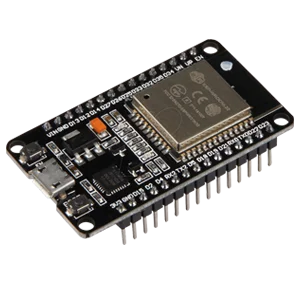
\includegraphics[width=\textwidth]{esp32devkit.png}
			\caption{ESP32 DevKit V1}
		\end{subfigure}
		\hfill
		\begin{subfigure}[b]{0.47\textwidth}
			\centering
			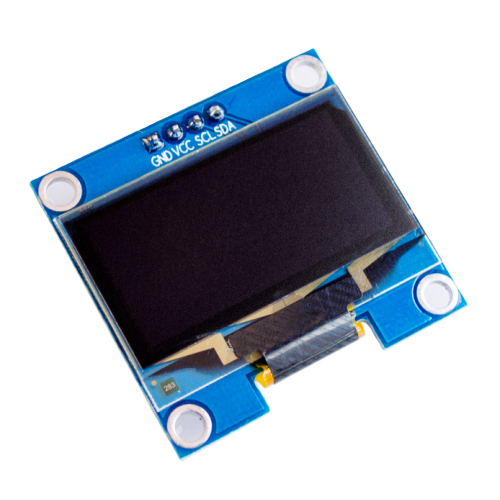
\includegraphics[width=\textwidth]{oled_display.png}
			\caption{SSD1306 OLED display}
		\end{subfigure}
		\caption{Core controller and display components}
		\label{fig:component-set-1}
	\end{figure}
	
	\begin{figure}[H]
		\centering
		\begin{subfigure}[b]{0.31\textwidth}
			\centering
			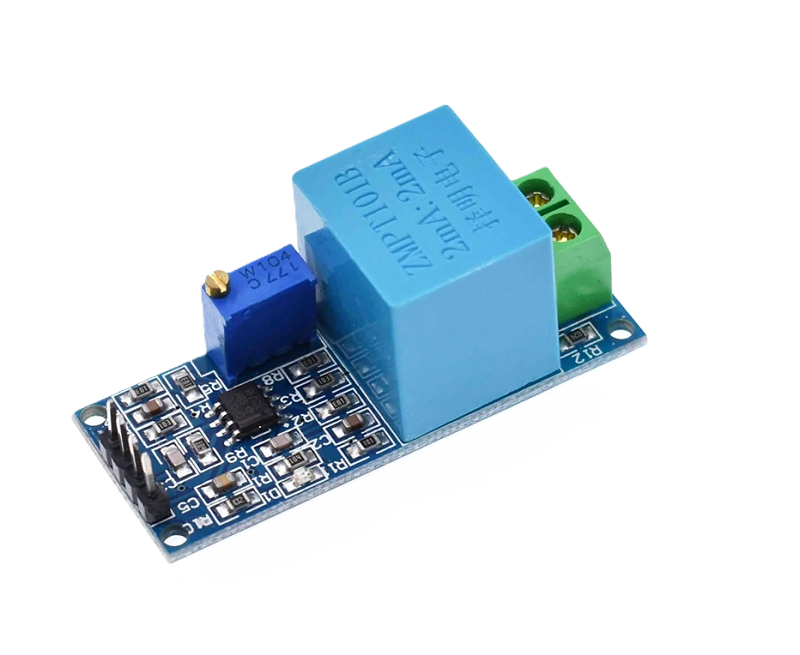
\includegraphics[width=\textwidth]{ZMPT101B_ac.png}
			\caption{ZMPT101B voltage sensor}
		\end{subfigure}
		\hfill
		\begin{subfigure}[b]{0.31\textwidth}
			\centering
			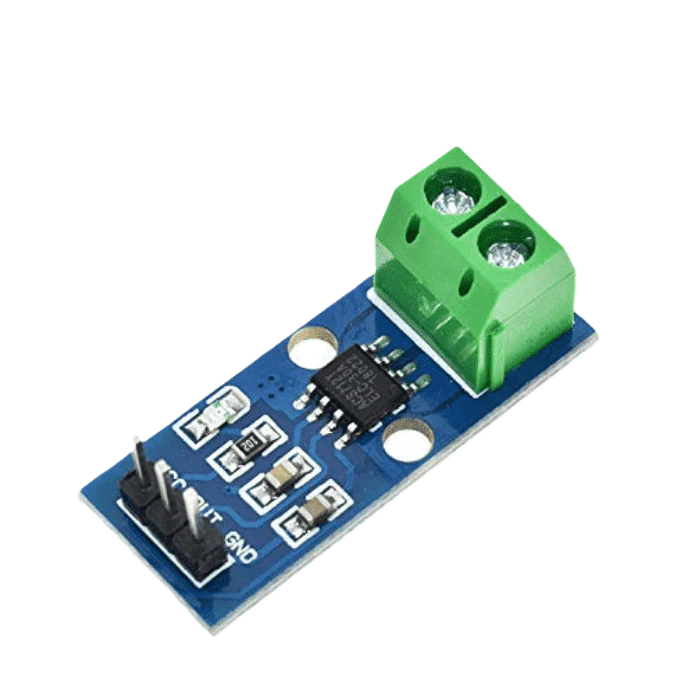
\includegraphics[width=\textwidth]{ACS712.png}
			\caption{ACS712 current sensor}
		\end{subfigure}
		\hfill
		\begin{subfigure}[b]{0.31\textwidth}
			\centering
			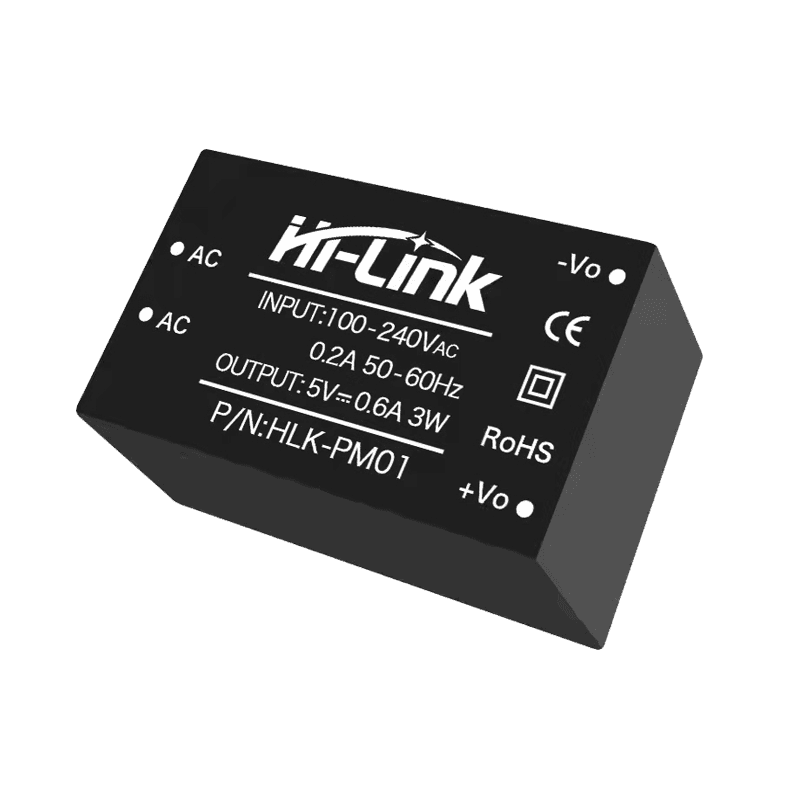
\includegraphics[width=\textwidth]{HLKPM01.png}
			\caption{HLK-PM01 power module}
		\end{subfigure}
		
		\vspace{0.35cm}
		
		\begin{subfigure}[b]{0.31\textwidth}
			\centering
			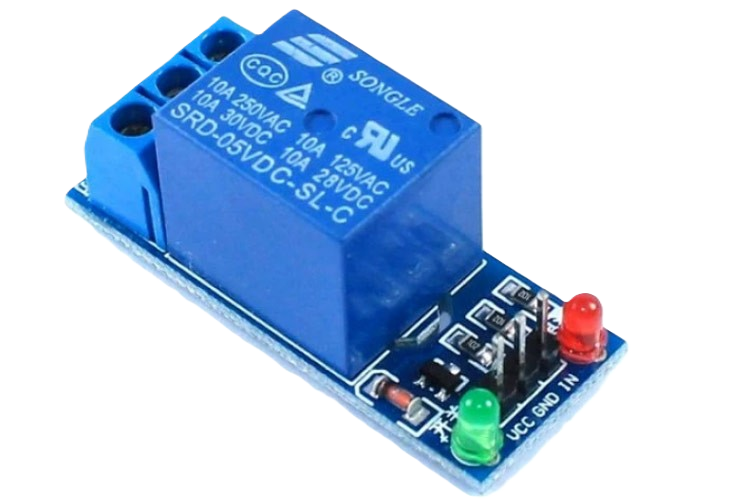
\includegraphics[width=\textwidth]{5V-relay.png}
			\caption{5V relay module}
		\end{subfigure}
		\hfill
		\begin{subfigure}[b]{0.31\textwidth}
			\centering
			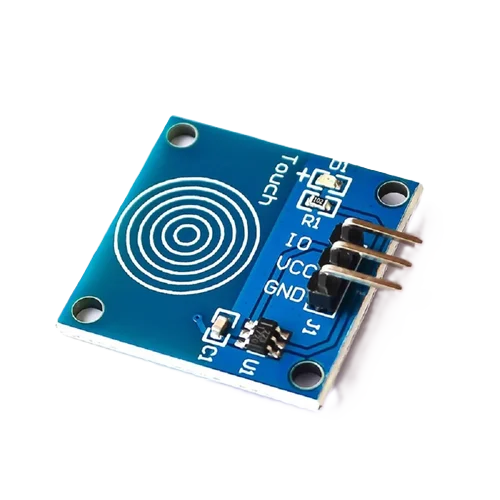
\includegraphics[width=\textwidth]{ttp223.png}
			\caption{TTP223 touch sensor}
		\end{subfigure}
		\caption{Sensing, power, and control modules used in the prototype}
		\label{fig:component-set-2}
	\end{figure}
	
	Using these exact modules kept the build practical and reproducible: the sensing pair (ZMPT101B + ACS712) gives measurable electrical input, HLK-PM01 provides isolated low-voltage supply, and relay plus TTP223 provides direct user control.
	
	\subsection{Software Specifications}
	
	The software stack consists of firmware running on the ESP32 and a backend server application. Fig.~\ref{fig:software-stack} shows the relationship between components.
	
	\begin{figure}[H]
		\centering
		\begin{tikzpicture}[
			node distance=0.5cm,
			component/.style={rectangle, draw, minimum width=2.5cm, minimum height=0.8cm, align=center, font=\footnotesize, rounded corners=2pt},
			layer/.style={rectangle, draw, dashed, minimum width=8cm, minimum height=1.5cm, align=center}
		]
		% Firmware layer
		\node[component, fill=primaryblue!20] (mp) {MicroPython};
		\node[component, fill=primaryblue!20, right=0.3cm of mp] (mqtt-fw) {umqtt};
		\node[component, fill=primaryblue!20, right=0.3cm of mqtt-fw] (ssd) {ssd1306};
		
		% Backend layer
		\node[component, fill=secondarygreen!20, below=1cm of mp] (flask) {Flask};
		\node[component, fill=secondarygreen!20, right=0.3cm of flask] (paho) {paho-mqtt};
		\node[component, fill=secondarygreen!20, right=0.3cm of paho] (lgbm) {LightGBM};
		
		% Frontend layer
		\node[component, fill=warnorange!20, below=1cm of flask] (html) {HTML/CSS};
		\node[component, fill=warnorange!20, right=0.3cm of html] (chartjs) {Chart.js};
		\node[component, fill=warnorange!20, right=0.3cm of chartjs] (sse) {SSE Client};
		
		% Labels
		\node[left=0.5cm of mp, font=\footnotesize\bfseries] {Firmware};
		\node[left=0.5cm of flask, font=\footnotesize\bfseries] {Backend};
		\node[left=0.5cm of html, font=\footnotesize\bfseries] {Frontend};
		\end{tikzpicture}
		\caption{Software stack components}
		\label{fig:software-stack}
	\end{figure}
	
	Figure~\ref{fig:software-stack} shows how responsibilities are split across firmware, backend, and frontend. This separation keeps device logic lightweight while still allowing richer analytics and visualization on the server side.
	
	\textbf{Firmware:} The firmware runs MicroPython 1.23 on the ESP32 DevKit V1. MicroPython was selected over C/Arduino because it speeds up prototyping, supports interactive REPL debugging, includes useful libraries for MQTT and I2C workflows, and allows quick iteration without full recompilation on each change.
	
	\textbf{Backend:} The server runs Python 3.11 with Flask for HTTP endpoints. The paho-mqtt library handles MQTT subscriptions. NanoMQ serves as a lightweight MQTT broker that runs on low-resource servers.
	
	\textbf{Frontend:} The web dashboard uses HTML, CSS, and JavaScript. Chart.js renders the historical power graph. Server-Sent Events (SSE) push live data to the browser without polling.
	
	\begin{table}[H]
		\centering
		\caption{Software stack summary}
		\label{tab:software}
		\vspace{6pt}
		\small
		\begin{tabularx}{\textwidth}{|p{3.0cm}|p{3.1cm}|X|}
			\hline
			\textbf{Layer} & \textbf{Technology} & \textbf{Purpose} \\
			\hline
			Firmware & MicroPython 1.23 & Sensor reading, RMS calculation, and MQTT publish/subscribe support \\
			Backend framework & Flask 3.0 & HTTP API services, relay commands, and SSE streaming \\
			MQTT client & paho-mqtt & Subscription and publish handling for telemetry and relay topics \\
			MQTT broker & NanoMQ & Message routing between edge devices and backend consumers \\
			ML libraries & LightGBM, scikit-learn & Power prediction, ON/OFF classification, and anomaly detection \\
			Frontend charts & Chart.js 4.4 & Historical and live trend visualization in dashboard panels \\
			\hline
		\end{tabularx}
		\normalsize
	\end{table}
	
	\subsection{Machine Learning Algorithm}
	
	The backend runs three machine learning models to analyze energy consumption patterns. Fig.~\ref{fig:ml-pipeline} shows how data flows through the ML pipeline.
	
	\begin{figure}[H]
		\centering
		\begin{tikzpicture}[
			node distance=1.2cm,
			block/.style={rectangle, draw, fill=gray!10, minimum width=2cm, minimum height=0.8cm, align=center, font=\footnotesize, rounded corners=2pt},
			model/.style={rectangle, draw, fill=secondarygreen!20, minimum width=2.5cm, minimum height=0.8cm, align=center, font=\footnotesize, rounded corners=2pt},
			arrow/.style={-{Stealth[length=2mm]}, thick}
		]
		\node[block] (input) {Telemetry\\Data};
		\node[block, right=of input] (features) {Feature\\Extraction};
		\node[model, right=of features] (predictor) {Power\\Predictor};
		\node[model, below=0.6cm of predictor] (classifier) {On/Off\\Classifier};
		\node[model, below=0.6cm of classifier] (anomaly) {Anomaly\\Detector};
		\node[block, right=of classifier] (output) {Dashboard\\Alert};
		
		\draw[arrow] (input) -- (features);
		\draw[arrow] (features) -- (predictor);
		\draw[arrow] (features) |- (classifier);
		\draw[arrow] (features) |- (anomaly);
		\draw[arrow] (predictor) -| (output);
		\draw[arrow] (classifier) -- (output);
		\draw[arrow] (anomaly) -| (output);
		\end{tikzpicture}
		\caption{ML pipeline data flow}
		\label{fig:ml-pipeline}
	\end{figure}
	
	Figure~\ref{fig:ml-pipeline} shows the backend inference path. Each telemetry packet is transformed into features, passed through prediction and classification models, and finally evaluated for anomaly flags before alert output.
	
	\textbf{Power predictor (LightGBM regression):} This model predicts expected power from time features (hour, weekday, month, season), lag features (1, 6, and 24-hour history), and rolling statistics (6-hour and 24-hour means).
	
	LightGBM (Light Gradient Boosting Machine) is a gradient boosting framework that builds an ensemble of decision trees. It performs well on tabular data with temporal patterns.
	
	\textbf{On/off classifier (LightGBM binary classification):} This model predicts whether an appliance should be on or off at a given time. It uses the same feature set as the power predictor. The training data has class imbalance (appliances are off more often than on), so we apply class weights during training to compensate.
	
	\textbf{Anomaly detector (Isolation Forest + Z-score):} This detector combines two checks. Isolation Forest catches structural outliers by measuring how easily a point gets isolated in random trees. Z-score catches sudden spikes by checking distance from the running mean.
	
	\textbf{What these ML algorithms do in this project:} LightGBM is a tree-based boosting method where each new tree corrects the error left by the previous trees. In regression mode, it predicts expected power in watts. In binary mode, it predicts whether the appliance is likely to be ON in the next hour. Isolation Forest does not need labeled anomaly samples; it learns normal behavior and flags points that are easier to isolate than typical observations.
	
	\begin{table}[H]
		\centering
		\caption{ML algorithms and their role in this system}
		\label{tab:ml-algorithm-role}
		\vspace{6pt}
		\small
		\begin{tabularx}{\textwidth}{|p{3.2cm}|p{5.0cm}|X|}
			\hline
			\textbf{Algorithm} & \textbf{Core idea} & \textbf{How it is used here} \\
			\hline
			LightGBM regression & Boosted decision trees minimize prediction error over continuous target values & Trained on hourly appliance features to estimate expected power for the next hour. Output is used in dashboard trend and prediction panels. \\
			\hline
			LightGBM binary classification & Boosted decision trees produce class probabilities for ON vs OFF behavior & Trained with class weighting to handle ON/OFF imbalance. Output supports next-hour state prediction and scheduled control logic. \\
			\hline
			Isolation Forest & Random trees isolate unusual samples in fewer splits than normal samples & Trained per appliance with contamination set to 2\%. Combined with Z-score in backend for robust anomaly flags. \\
			\hline
		\end{tabularx}
		\normalsize
	\end{table}
	
	A reading is flagged if either method triggers. The contamination parameter is set to 2\%, meaning the model expects roughly 2\% of readings to be anomalous.
	
	\textbf{Training data:} The models are trained on the PLEGMA dataset \cite{plegma}, which provides domestic appliance-level and aggregate electricity demand along with environmental metadata from homes. For this project, the raw data is organized house-wise (e.g., \texttt{House\_01}, \texttt{House\_02}, \dots) and then converted into hourly learning tables used by the backend models.
	
	\begin{table}[H]
		\centering
		\caption{PLEGMA data elements used in this project}
		\label{tab:plegma-elements}
		\vspace{6pt}
		\begin{tabular}{|l|p{5.2cm}|p{4.1cm}|}
			\hline
			\textbf{Source} & \textbf{Columns used} & \textbf{Use in pipeline} \\
			\hline
			Electric data files & Appliance channels (\texttt{ac\_1}, \texttt{fridge}, \texttt{boiler}, etc.), aggregate power (\texttt{P\_agg}), \texttt{V}, \texttt{A}, quality flag (\texttt{issues}), timestamp & Target variables, ON/OFF detection, and quality filtering \\
			\hline
			Environmental files & \texttt{external\_temperature}, \texttt{internal\_temperature}, \texttt{external\_humidity}, \texttt{internal\_humidity}, timestamp & Context features for model robustness across season and weather \\
			\hline
			House metadata path & House ID from folder structure & Cross-house pooling while retaining source identity \\
			\hline
		\end{tabular}
	\end{table}
	
	The raw electric series is recorded at short intervals (approximately 10s cadence in the imported files), then rolled up to hourly windows for stable model training. This gives a good balance between preserving usage behavior and reducing noise from second-level fluctuations.
	
	\begin{table}[H]
		\centering
		\caption{ML model performance metrics}
		\label{tab:ml-metrics}
		\vspace{6pt}
		\begin{tabular}{|l|l|r|}
			\hline
			\textbf{Model} & \textbf{Metric} & \textbf{Value} \\
			\hline
			Power predictor & R\textsuperscript{2} score & 0.87 \\
			\hline
			On/off classifier & Accuracy & 94\% \\
			\hline
			Anomaly detector & Precision & 89\% \\
			\hline
		\end{tabular}
	\end{table}
	
	\subsection{Cloud Platform}
	
	The system deploys to a DigitalOcean droplet running Ubuntu 22.04. A \$6/month instance (1 vCPU, 1GB RAM) is enough for NanoMQ brokering, Flask APIs with ML inference, and static dashboard hosting in this prototype setup.
	
	The deployment uses a simple setup without reverse proxy or SSL encryption for the development phase. Flask runs directly on port 5000. The deployment script (\texttt{deploy.sh}) automates dependency installation and service configuration.
	
	\subsection{Development Tools}
	
	Development work used VS Code (with Python and MicroPython extensions), ampy for serial file upload to ESP32 flash, esptool.py for firmware flashing, Git/GitHub for version control, MQTT Explorer for message inspection, and Jupyter Notebook for model experiments.
	
	\subsection{GitHub Link}
	
	The complete source code is available at:
	
	\url{https://github.com/lostfleetdev/Smart-Energy-Meter-IOT}
	
	\newpage
	
	\section{Project Design / Methodology}\label{sec:design}
	
	\subsection{System Architecture}
	
	The system follows a three-tier IoT architecture: edge device, backend server, and web frontend. Fig.~\ref{fig:architecture} shows how data flows between the tiers.
	
	\begin{figure}[H]
		\centering
		\resizebox{0.90\textwidth}{!}{%
		\begin{tikzpicture}[
			group/.style={rectangle, draw, rounded corners=6pt, minimum width=4.1cm, minimum height=6.2cm},
			module/.style={rectangle, draw, rounded corners=2pt, fill=white, text width=3.2cm, minimum height=0.62cm, align=center, font=\scriptsize, inner sep=2pt},
			arrow/.style={-{Stealth[length=2.5mm]}, thick}
		]
		% Layer containers
		\node[group, fill=primaryblue!12] (device) at (0,0) {};
		\node[group, fill=secondarygreen!12] (server) at (5.4,0) {};
		\node[group, fill=warnorange!12] (browser) at (10.8,0) {};
		
		% Layer titles
		\node[font=\small\bfseries] at ([yshift=3.4cm]device.center) {Device layer (ESP32)};
		\node[font=\small\bfseries] at ([yshift=3.4cm]server.center) {Server layer (Cloud VM)};
		\node[font=\small\bfseries] at ([yshift=3.4cm]browser.center) {Browser layer};
		
		% Device modules
		\node[module] (d_sense) at ([yshift=2.2cm]device.center) {Sensor readout\\(voltage and current)};
		\node[module] (d_calc) at ([yshift=1.2cm]device.center) {RMS and power\\computation};
		\node[module] (d_oled) at ([yshift=0.2cm]device.center) {Local OLED update};
		\node[module] (d_pub) at ([yshift=-0.8cm]device.center) {MQTT publish\\/telemetry};
		\node[module] (d_sub) at ([yshift=-1.8cm]device.center) {MQTT subscribe\\/relay/set};
		
		% Server modules
		\node[module] (s_broker) at ([yshift=2.4cm]server.center) {NanoMQ broker};
		\node[module] (s_ingest) at ([yshift=1.4cm]server.center) {Flask ingestion service};
		\node[module] (s_ml) at ([yshift=0.2cm]server.center) {ML inference\\(LightGBM, Isolation Forest)};
		\node[module] (s_store) at ([yshift=-1cm]server.center) {CSV data storage};
		\node[module] (s_api) at ([yshift=-2cm]server.center) {REST and SSE endpoints};
		
		% Browser modules
		\node[module] (b_dash) at ([yshift=2.4cm]browser.center) {Live dashboard};
		\node[module] (b_hist) at ([yshift=0.2cm]browser.center) {Charts and history};
		\node[module] (b_ctrl) at ([yshift=-1.2cm]browser.center) {Relay control panel};
		
		% Data and control flow
		\draw[arrow] (d_pub.east) -- node[above, font=\scriptsize] {MQTT telemetry} (s_broker.west);
		\draw[arrow] (s_broker.south) -- (s_ingest.north);
		\draw[arrow] (s_ingest.south) -- (s_ml.north);
		\draw[arrow] (s_ml.south) -- (s_store.north);
		\draw[arrow] (s_store.east) -- node[above, font=\scriptsize] {History data} (b_hist.west);
		\draw[arrow] (s_api.east) -- node[above, font=\scriptsize] {SSE updates} (b_dash.west);
		\draw[arrow] (b_ctrl.west) -- node[below, font=\scriptsize] {REST request} (s_api.east);
		\draw[arrow, dashed] (s_api.west) -- node[below, font=\scriptsize] {MQTT relay command} (d_sub.east);
		\end{tikzpicture}%
		}
		\caption{Detailed system architecture showing module-level data and control flow}
		\label{fig:architecture}
	\end{figure}
	
	As shown in Fig.~\ref{fig:architecture}, the system is organized into three layers with clear responsibilities. The device layer acquires electrical signals, computes measurement values, and exchanges MQTT messages. The server layer manages message brokering, telemetry processing, machine learning inference, and data storage. The browser layer displays live and historical information and sends relay control requests, which return to the device through the server control path.
	
	Device layer (ESP32 DevKit V1): The ESP32 samples voltage and current at 200 points per cycle, computes RMS values and power factor, publishes JSON telemetry through MQTT, updates the local OLED, and handles touch input for relay control.
	
	Backend layer (Flask + NanoMQ): NanoMQ receives MQTT traffic from devices. Flask processes telemetry, runs ML inference per reading, stores CSV history, and pushes dashboard updates through SSE.
	
	Frontend layer (Web dashboard): The web interface shows live readings and historical charts, lets users switch relay state, and updates in real time through SSE without polling.
	
	\subsection{Modules of the System}
	
	The system works through five modules. The sensing module uses ZMPT101B and ACS712 signals on ESP32 ADC pins and applies calibration to get stable voltage and current values. The processing module samples one full AC cycle (200 points over 20ms), computes square sums, derives RMS values with $V_{RMS} = \sqrt{\frac{1}{N}\sum v_i^2}$, estimates phase relationship, and integrates power for energy tracking. The communication module publishes sensor telemetry to \texttt{energy/\{device\_id\}/telemetry} and listens for relay commands on \texttt{energy/\{device\_id\}/relay/set}. The intelligence module loads trained \texttt{.pkl} artifacts and performs regression, classification, and anomaly checks on incoming records. The interface module exposes local OLED screens and a remote dashboard with charts plus relay controls.
	
	\subsection{Circuit Diagram}
	
	Fig.~\ref{fig:circuit} shows the complete circuit diagram of the Smart Energy Meter. The connections are described in Table~\ref{tab:gpio}.
	
	\begin{figure}[H]
		\centering
		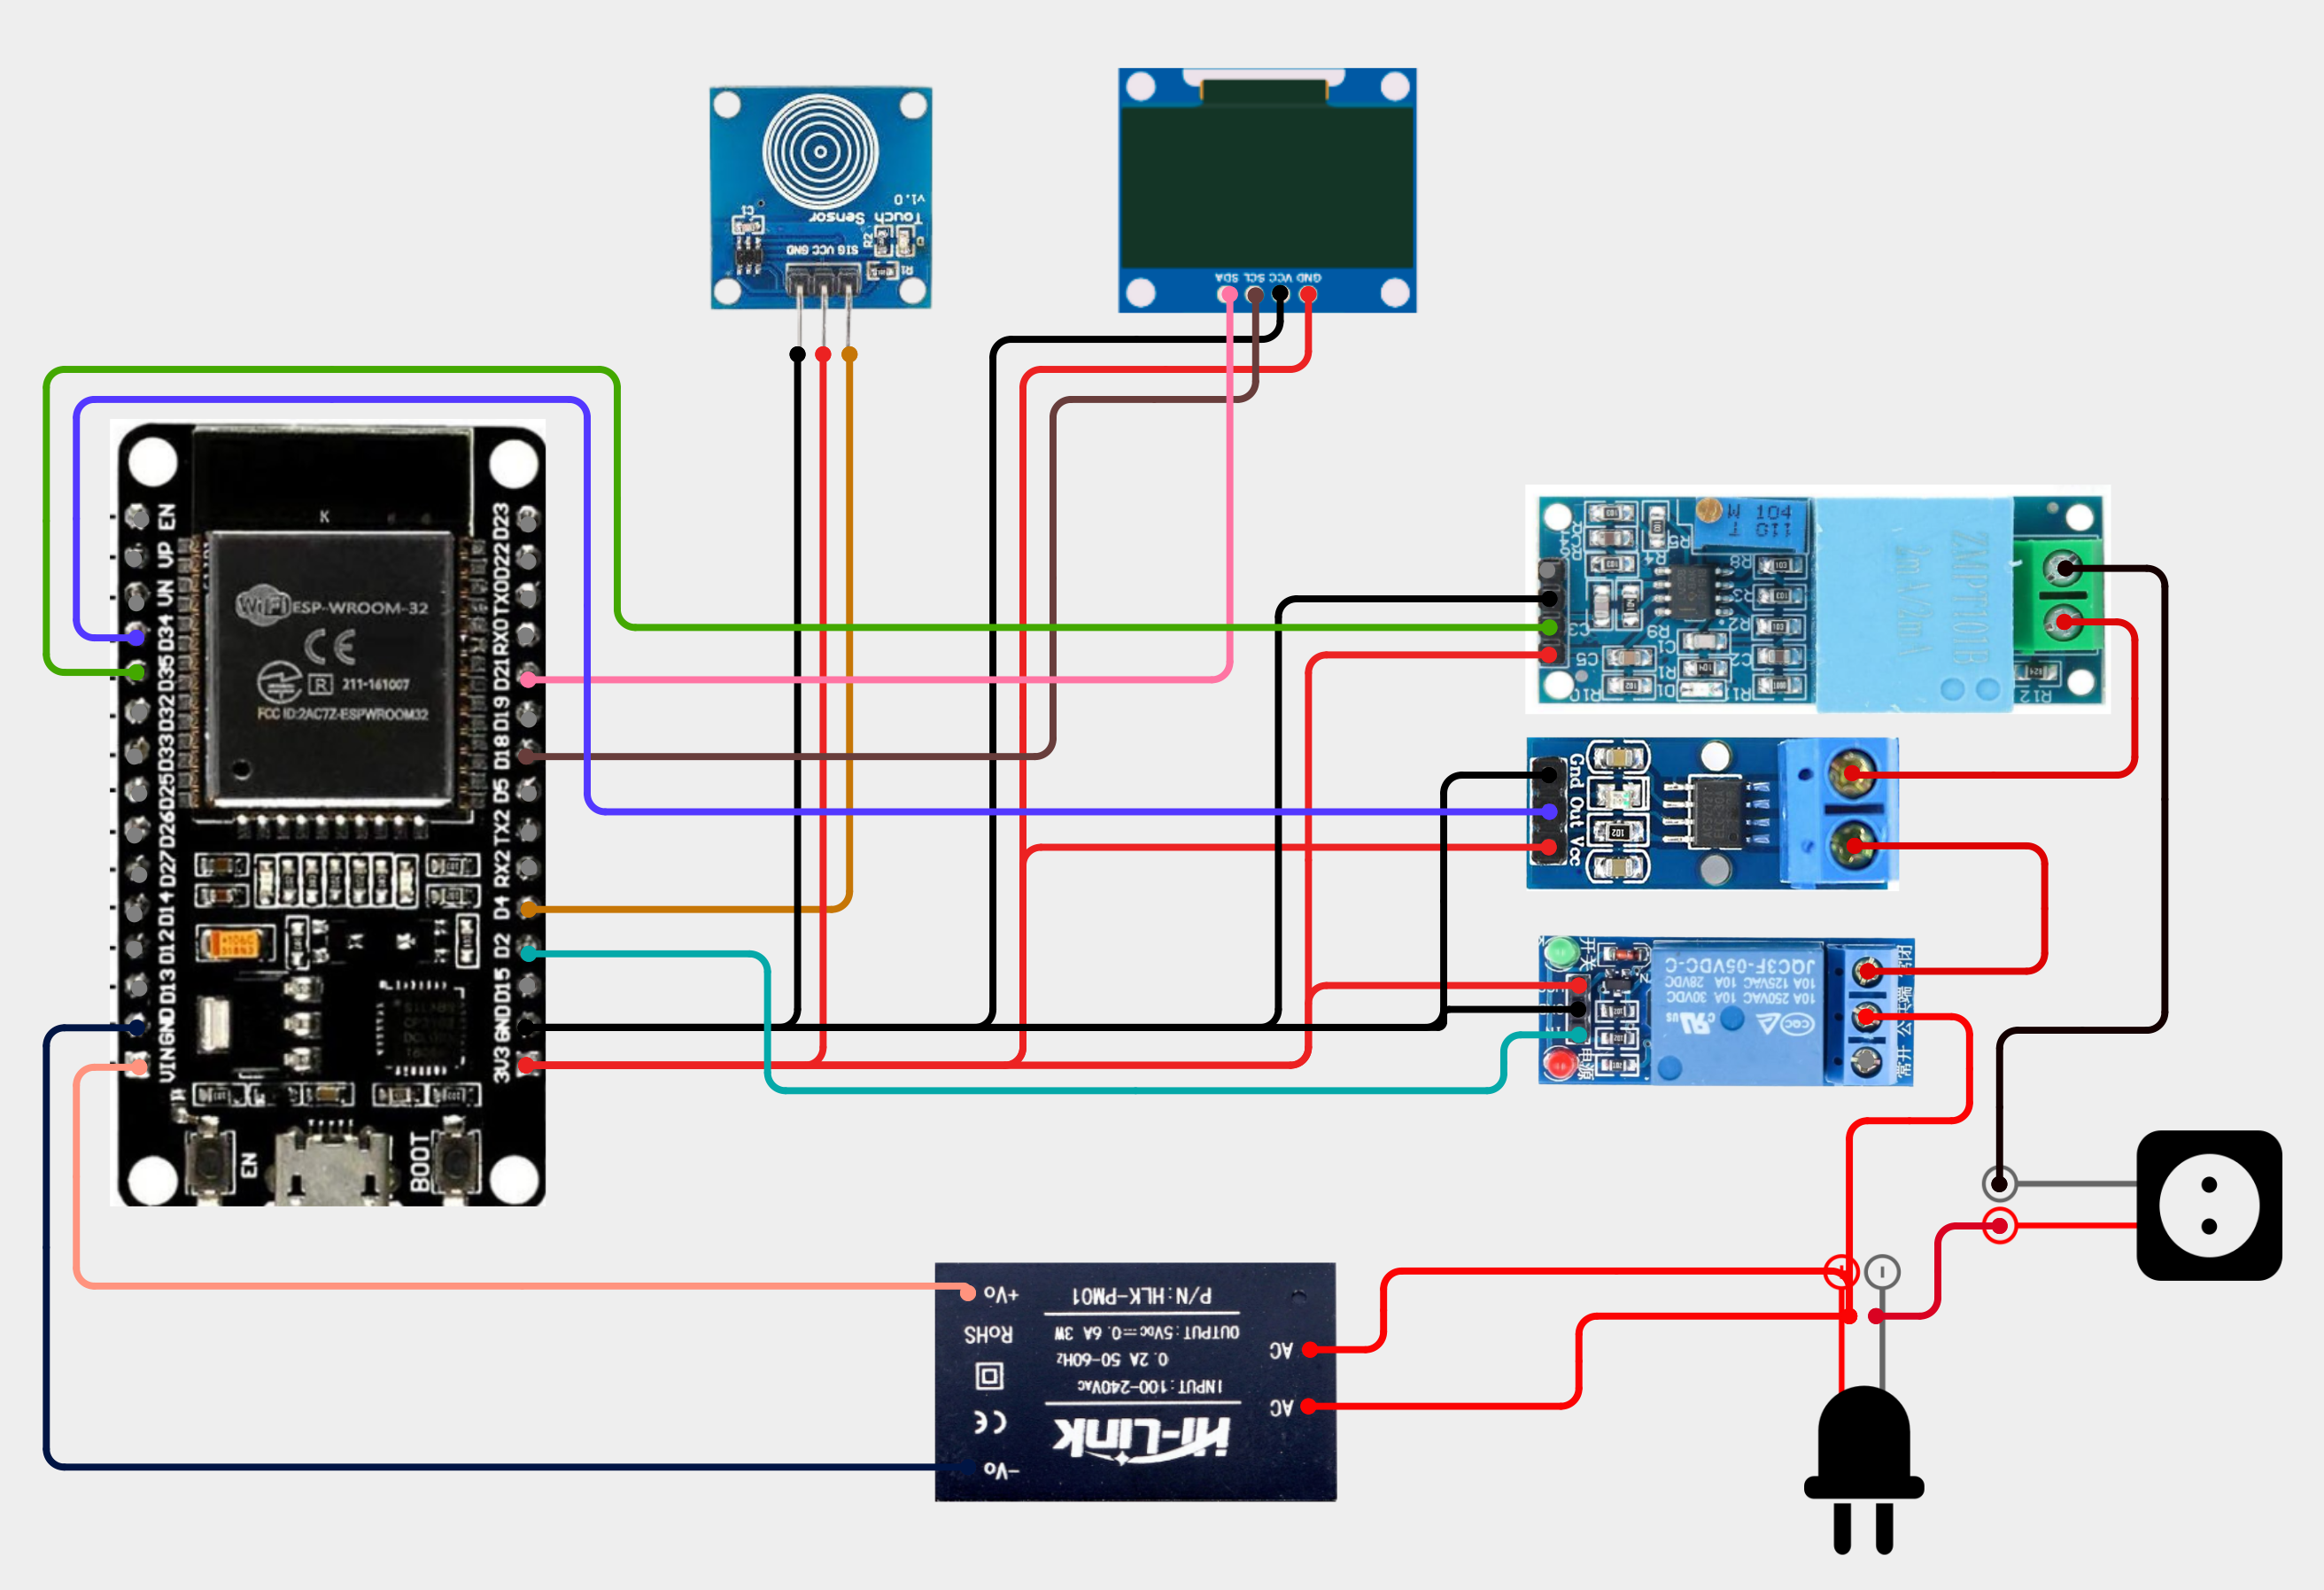
\includegraphics[width=0.90\textwidth]{circuit_image.png}
		\caption{Circuit diagram of the Smart Energy Meter}
		\label{fig:circuit}
	\end{figure}
	
	Figure~\ref{fig:circuit} presents the final electrical connections used in the prototype. It captures the sensing path, control path, and supply path clearly, which helps during assembly, troubleshooting, and safety checks before powering the load.
	
	\subsection{Connections}
	
	\begin{table}[H]
		\centering
		\caption{GPIO pin assignments}
		\label{tab:gpio}
		\vspace{6pt}
		\begin{tabular}{|c|l|l|l|}
			\hline
			\textbf{GPIO} & \textbf{Function} & \textbf{Direction} & \textbf{Connected to} \\
			\hline
			35 & Voltage ADC & Input & ZMPT101B output \\
			34 & Current ADC & Input & ACS712 output \\
			18 & I2C SCL & Output & OLED clock \\
			21 & I2C SDA & Bidirectional & OLED data \\
			2 & Relay control & Output & Relay IN (active LOW) \\
			4 & Touch sensor & Input & TTP223 output \\
			\hline
		\end{tabular}
	\end{table}
	
	\textbf{Power connection:} The HLK-PM01 converts 230V AC mains to 5V DC. On the ESP32 board, the AMS1117-3.3V regulator provides 3.3V for logic and sensing.
	
	\textbf{Voltage sensing connection:} The ZMPT101B output is connected to GPIO 35 (ADC input). Its conditioned signal is centered near VCC/2, allowing RMS voltage computation.
	
	\textbf{Current sensing connection:} The ACS712-20A output is connected to GPIO 34 (ADC input), where current is measured through its Hall-effect output signal.
	
	\textbf{Display and control connections:} The SSD1306 OLED is connected through I2C (GPIO 18 as SCL and GPIO 21 as SDA). The relay input is connected to GPIO 2, and the TTP223 touch output is connected to GPIO 4 for local control.
	
	\subsection{Machine Learning}
	
	The ML pipeline processes historical energy data through four stages. Fig.~\ref{fig:ml-stages} shows the data transformation at each stage.
	
	\begin{figure}[H]
		\centering
		\resizebox{0.94\textwidth}{!}{%
		\begin{tikzpicture}[
			node distance=0.75cm,
			stage/.style={rectangle, draw, rounded corners=3pt, minimum width=2.6cm, minimum height=0.85cm, align=center, font=\footnotesize},
			arrow/.style={-{Stealth[length=2mm]}, thick, draw=black!70}
		]
		\node[stage, fill=primaryblue!15] (load) {Data\\Loading};
		\node[stage, fill=secondarygreen!15, right=of load] (clean) {Cleaning};
		\node[stage, fill=warnorange!15, right=of clean] (agg) {Aggregation};
		\node[stage, fill=gray!18, right=of agg] (feat) {Feature\\Engineering};
		\node[stage, fill=primaryblue!15, right=of feat] (train) {Training};
		
		\draw[arrow] (load) -- (clean);
		\draw[arrow] (clean) -- (agg);
		\draw[arrow] (agg) -- (feat);
		\draw[arrow] (feat) -- (train);
		
		% Labels below
		\node[below=0.3cm of load, font=\scriptsize, align=center] {CSV files\\(raw)};
		\node[below=0.3cm of clean, font=\scriptsize, align=center] {Issues filter\\+ outlier trim};
		\node[below=0.3cm of agg, font=\scriptsize, align=center] {Hourly\\rollup};
		\node[below=0.3cm of feat, font=\scriptsize, align=center] {Lag + rolling\\+ calendar};
		\node[below=0.3cm of train, font=\scriptsize, align=center] {LightGBM +\\Isolation Forest};
		\end{tikzpicture}%
		}
		\caption{ML pipeline stages}
		\label{fig:ml-stages}
	\end{figure}
	
	The training pipeline begins by loading PLEGMA house folders and merging electric data with environmental data on timestamp. The data is then cleaned with rule-based filters: rows marked by \texttt{issues} are dropped, missing appliance targets are removed, negative values are rejected, and extreme values above the 99.9th percentile are clipped. Short gaps are forward-filled up to six readings to preserve local continuity without creating long synthetic segments.
	
	After cleaning, all records are grouped into hourly windows. For each appliance, the pipeline computes hourly mean, max, min, and standard deviation, plus ON-duration indicators and optional environmental averages. This step improved consistency during training, especially for intermittent loads like washing machines and dishwashers.
	
	Feature engineering adds calendar context (hour, day-of-week, weekend, month, season, and time-period bins), lag terms (\texttt{lag\_1}, \texttt{lag\_2}, \texttt{lag\_3}, \texttt{lag\_6}, \texttt{lag\_12}, \texttt{lag\_24}), rolling terms (6h and 24h means), and difference terms (\texttt{diff\_1h}, \texttt{diff\_24h}). The final split is time-ordered (80\% train, 20\% test), which mirrors real deployment where future behavior must be predicted from past data.
	
	\begin{table}[H]
		\centering
		\caption{Appliance-specific data selection in the training pipeline}
		\label{tab:quality-houses}
		\vspace{6pt}
	\small
	\setlength{\tabcolsep}{4pt}
	\begin{tabularx}{\textwidth}{|p{1.8cm}|p{3.3cm}|p{1.9cm}|X|}
			\hline
			\textbf{Appliance} & \textbf{Selected houses} & \textbf{ON threshold (W)} & \textbf{Dataset type for regression} \\
			\hline
			AC 1 & 1, 3, 7, 2, 11 & 100 & Active-hours preferred \\
			\hline
			AC 2 & 3, 1, 7, 11 & 100 & Active-hours preferred \\
			\hline
			Boiler & 1, 4, 7, 9, 2 & 200 & Active-hours preferred \\
			\hline
			Fridge & 1, 3, 7, 8, 6 & 30 & Full-hour dataset \\
			\hline
			Washing machine & 7, 12, 5, 3 & 50 & Active-hours preferred \\
			\hline
			Dishwasher & 12 & 20 & Full-hour fallback when active set is small \\
			\hline
		\end{tabularx}
		\setlength{\tabcolsep}{6pt}
		\normalsize
	\end{table}
	
	For classification, the target is defined as ``next-hour ON'' using the next hour's ON ratio (\texttt{target\_on = next\_hour\_on > 0.3}). This keeps labels practical for real scheduling behavior. For anomaly detection, Isolation Forest is trained with contamination fixed at 2\%, and the backend combines it with a Z-score rule so both structural and sudden deviations are captured.
	
	\subsubsection{ML implementation in project code}
	
	In training, the regression model uses LightGBM with regression objective, MAE metric, and early stopping after 50 rounds without validation improvement. The classifier uses LightGBM in binary mode, applies class weighting, and tunes the decision threshold by scanning probability cutoffs to maximize F1 score. The anomaly model uses StandardScaler with Isolation Forest (200 estimators and 2\% contamination).
	
	Each trained artifact is exported as a \texttt{.pkl} file with model object, feature list, and runtime metadata (for example threshold, training metrics, or anomaly statistics). This structure is important because the backend must apply features in exactly the same order used during training.
	
	\begin{table}[H]
		\centering
		\caption{Training stage vs runtime stage in ML implementation}
		\label{tab:ml-implementation-stages}
		\vspace{6pt}
		\footnotesize
		\begin{tabularx}{\textwidth}{|p{3.3cm}|p{4.1cm}|X|}
			\hline
			\textbf{Stage} & \textbf{Code location} & \textbf{What happens} \\
			\hline
			Data preparation & ML/data\_pipeline.py & House-level CSV load, issue filtering, outlier clipping, hourly aggregation, lag and rolling feature creation, and export of processed datasets. \\
			\hline
			Model training & ML/train\_models.py & LightGBM regressor and classifier training with time-based split (80/20), early stopping, threshold tuning, and Isolation Forest fitting. \\
			\hline
			Model loading & backend/ml\_service.py & Startup loading of .pkl artifacts into memory for each appliance model family. \\
			\hline
			Live feature build & backend/ml\_service.py & Runtime feature extraction from recent history deque: hour, weekday, lag\_1h, lag\_24h, diff\_1h, diff\_24h, rolling mean/std. \\
			\hline
			Inference and API output & backend/main.py + backend/ml\_service.py & Prediction, ON/OFF classification, and anomaly checks are served through REST routes and integrated with dashboard updates. \\
			\hline
		\end{tabularx}
		\normalsize
	\end{table}
	
	\subsubsection{How trained models are used at runtime}
	
	At runtime, each incoming telemetry message updates appliance history first. The backend then builds the latest feature vector and runs three operations: expected power prediction, ON/OFF state probability, and anomaly decision. If model history is too short, the service returns an explicit ``insufficient history'' error rather than emitting an unreliable prediction. This behavior keeps dashboard output honest during startup or after long connection gaps.
	
	\newpage
	
	\section{Implementation / Working}\label{sec:implementation}
	
	\subsection{Working Flow}
	
	The following sequence diagram (Fig.~\ref{fig:sequence}) shows the data flow from sensor reading to dashboard display. Solid arrows indicate the telemetry path; dashed arrows indicate the relay control path.
	
	\begin{figure}[H]
		\centering
		\resizebox{0.90\textwidth}{!}{%
		\begin{tikzpicture}[
			node distance=1cm,
			participant/.style={rectangle, draw, minimum height=0.7cm, minimum width=1.6cm, font=\footnotesize},
			arrow/.style={-{Stealth[length=2mm]}, thick},
			msg/.style={font=\scriptsize},
			lifeline/.style={dashed, gray}
		]
		
		% Participants
		\node[participant] (sensors) {Sensors};
		\node[participant, right=1.2cm of sensors] (esp) {ESP32};
		\node[participant, right=1.2cm of esp] (mqtt) {NanoMQ};
		\node[participant, right=1.2cm of mqtt] (backend) {Backend};
		\node[participant, right=1.2cm of backend] (dash) {Dashboard};
		
		% Lifelines
		\draw[lifeline] (sensors.south) -- ++(0,-8);
		\draw[lifeline] (esp.south) -- ++(0,-8);
		\draw[lifeline] (mqtt.south) -- ++(0,-8);
		\draw[lifeline] (backend.south) -- ++(0,-8);
		\draw[lifeline] (dash.south) -- ++(0,-8);
		
		% Messages - Telemetry path
		\draw[arrow] ($(sensors.south)+(0,-0.6)$) -- node[above, msg] {ADC read} ($(esp.south)+(0,-0.6)$);
		\draw[arrow] ($(esp.south)+(0,-1.2)$) -- node[above, msg] {RMS calc} ($(esp.south)+(0.2,-1.2)$);
		\draw[arrow] ($(esp.south)+(0,-1.8)$) -- node[above, msg] {MQTT pub} ($(mqtt.south)+(0,-1.8)$);
		\draw[arrow] ($(mqtt.south)+(0,-2.4)$) -- node[above, msg] {Forward} ($(backend.south)+(0,-2.4)$);
		\draw[arrow] ($(backend.south)+(0,-3.0)$) -- node[above, msg] {Parse JSON} ($(backend.south)+(0.2,-3.0)$);
		\draw[arrow] ($(backend.south)+(0,-3.6)$) -- node[above, msg] {ML infer} ($(backend.south)+(0.2,-3.6)$);
		\draw[arrow] ($(backend.south)+(0,-4.2)$) -- node[above, msg] {Store CSV} ($(backend.south)+(0.2,-4.2)$);
		\draw[arrow] ($(backend.south)+(0,-4.8)$) -- node[above, msg] {SSE push} ($(dash.south)+(0,-4.8)$);
		\draw[arrow] ($(dash.south)+(0,-5.4)$) -- node[above, msg] {Update UI} ($(dash.south)+(0.2,-5.4)$);
		
		% Return path for relay control
		\draw[arrow, dashed] ($(dash.south)+(0,-6.2)$) -- node[above, msg] {POST /relay} ($(backend.south)+(0,-6.2)$);
		\draw[arrow, dashed] ($(backend.south)+(0,-6.8)$) -- node[above, msg] {MQTT relay} ($(mqtt.south)+(0,-6.8)$);
		\draw[arrow, dashed] ($(mqtt.south)+(0,-7.4)$) -- node[above, msg] {Relay cmd} ($(esp.south)+(0,-7.4)$);
		
		\end{tikzpicture}%
		}
		\caption{System sequence diagram}
		\label{fig:sequence}
	\end{figure}
	
	The system runs in a repeating loop. First, the ESP32 boots, loads calibration values, joins WiFi, and starts MQTT. It then samples 200 voltage points and 200 current points over one 50Hz cycle, computes RMS values using $V_{RMS} = \sqrt{\frac{1}{n}\sum_{i=1}^{n} v_i^2}$, derives power, and integrates energy. The OLED is refreshed every second, and telemetry is published at the configured interval (default 5s). The backend parses each payload, runs ML inference, stores the record, and pushes updates over SSE. The dashboard refreshes live gauges and history, while relay control commands from either the touch input or web UI flow back through MQTT. This cycle keeps running while the device remains powered.
	
	\subsection{Calibration Process}
	
	Before deployment, each unit undergoes calibration to account for sensor variations. The process takes approximately 5 minutes and requires a known load (we used a 600W electric kettle).
	
	Step 1 is a no-load baseline pass: with no appliance connected, the relay closes and the firmware collects 2000 samples per channel to estimate midpoint offsets and noise floor. Step 2 is known-load scaling: the kettle is connected, five readings are averaged, and those values are matched against the 230V/600W reference to derive voltage and current scale factors. Step 3 saves the calibration constants to \texttt{calibration.json} and verifies the displayed values against a reference meter.
	
	The calibration output file has the following format:
	
	\begin{lstlisting}[basicstyle=\ttfamily\small, frame=single]
	{
	  "v_midpoint": 2965,
	  "v_scale": 0.2103,
	  "acs_midpoint_v": 2.373,
	  "acs_sensitivity": 0.1075,
	  "v_noise_threshold": 5.78,
	  "i_noise_threshold": 0.107
	}
	\end{lstlisting}
	
	\subsection{Firmware Operation}
	
	The firmware uses a tight 20ms timing loop with layered tasks. Sensor processing runs once per second with 200-point voltage/current sampling, RMS calculation, calibration scaling, and power/energy updates. OLED refresh also runs every second and changes screens on long touch input. Touch handling watches GPIO 4 continuously, where a short tap (50--600ms) toggles relay state and a long press advances the display. When relay state changes to OFF, auto-zero logic waits 300ms and re-estimates ACS712 baseline to reduce drift. MQTT publishing sends voltage, current, power, energy, and relay state in JSON at the configured interval.
	
	\subsection{Measured Parameters}
	
	Table \ref{tab:params} lists the electrical parameters measured and calculated by the system.
	
	\begin{table}[H]
		\centering
		\caption{Measured electrical parameters}
		\label{tab:params}
		\vspace{6pt}
		\begin{tabular}{|l|l|p{6cm}|}
			\hline
			\textbf{Metric} & \textbf{Formula} & \textbf{Description} \\
			\hline
			RMS Voltage & $\sqrt{\frac{1}{n}\sum v^2}$ & True voltage accounting for AC waveform \\
			RMS Current & $\sqrt{\frac{1}{n}\sum i^2}$ & True current with dynamic zero compensation \\
			Real Power & $V \times I \times PF$ & Actual power consumed (W) \\
			Apparent Power & $V \times I$ & Total power drawn from supply (VA) \\
			Power Factor & $\frac{\text{Real}}{\text{Apparent}}$ & Efficiency metric (0--1) \\
			Energy & $\int P \, dt$ & Cumulative consumption (kWh) \\
			\hline
		\end{tabular}
	\end{table}
	
	\subsection{Backend Data Interfaces}
	
	The implementation in \texttt{backend/main.py} uses a simple but clear interface design: MQTT for device messaging, REST endpoints for browser control and history access, and SSE for low-latency telemetry updates. This split keeps device communication lightweight while still exposing useful APIs to the dashboard.
	
	\begin{table}[H]
		\centering
		\caption{MQTT topics used in runtime operation}
		\label{tab:mqtt-topics}
		\vspace{6pt}
	\footnotesize
	\resizebox{\textwidth}{!}{%
	\begin{tabular}{|p{4.1cm}|p{2.7cm}|p{7.5cm}|}
			\hline
			\textbf{Topic} & \textbf{Direction} & \textbf{Role} \\
			\hline
			energy/\{device\_id\}/\allowbreak telemetry & Device to backend & Periodic payload carrying voltage, current, power, energy, and appliance tag \\
			\hline
			energy/\{device\_id\}/\allowbreak relay/set & Backend to device & Relay command ("1" for ON, "0" for OFF) issued from dashboard \\
			\hline
			energy/\{device\_id\}/\allowbreak relay/state & Device to backend & Device-side relay confirmation to keep UI state synchronized \\
			\hline
		\end{tabular}
	}
	\normalsize
	\end{table}
	
	\begin{table}[H]
		\centering
		\caption{Main backend endpoints used by dashboard and ML integration}
		\label{tab:backend-endpoints}
		\vspace{6pt}
	\footnotesize
	\resizebox{\textwidth}{!}{%
	\begin{tabular}{|p{3.9cm}|p{1.7cm}|p{8.6cm}|}
			\hline
			\textbf{Endpoint} & \textbf{Method} & \textbf{Purpose} \\
			\hline
			/stream & GET & SSE stream for live telemetry push without client polling \\
			\hline
			/history & GET & Returns recent CSV-backed records for charting \\
			\hline
			/relay & GET/POST & Reads relay state and publishes relay-set command \\
			\hline
			/stats & GET & Returns buffer statistics (avg/min/max power, client count) \\
			\hline
			/ml/predict/\allowbreak \{appliance\} & GET & Next-hour power prediction from LightGBM model \\
			\hline
			/ml/anomaly/\allowbreak \{appliance\} & POST & Anomaly decision from Isolation Forest + Z-score logic \\
			\hline
			/ml/reading/\allowbreak \{appliance\} & POST & Adds reading to ML history buffer and returns quick anomaly check \\
			\hline
		\end{tabular}
	}
		\normalsize
	\end{table}
	
	This interface design also supports fallback behavior. If a trained model is unavailable or there is insufficient history for prediction, the backend returns an explicit error response instead of silent defaults. That behavior helped debugging during integration and made dashboard status messages easier to interpret.
	
	\newpage
	\section{Result / Output}\label{sec:results}
	
	This section presents the outputs from each module of the system. The results include hardware implementation photos, web dashboard screenshots, ML model performance metrics, and measurement accuracy tests.
	
	\begin{table}[H]
		\centering
		\caption{Traceability between report modules and repository implementation}
		\label{tab:traceability}
		\vspace{6pt}
		\small
		\resizebox{\textwidth}{!}{%
		\begin{tabular}{|p{3.0cm}|p{4.0cm}|p{7.2cm}|}
			\hline
			\textbf{Module in report} & \textbf{Repository} & \textbf{Observed implementation} \\
			\hline
			Local sensing firmware & \url{device/main.py}, \url{device/calibrate.py} & RMS acquisition, OLED multi-screen view, touch control, relay switching, and calibration file workflow are implemented. \\
			\hline
			Network-enabled firmware path & \url{device/main_v2.py}, \url{device/boot_v2.py} & WiFi connection, MQTT publish/subscribe, telemetry packet construction, and remote relay callback handling are implemented in the v2 path. \\
			\hline
			Backend telemetry and control & \url{backend/main.py} & MQTT ingestion, CSV storage, SSE streaming, history APIs, and relay command endpoint are implemented and integrated in one Flask service. \\
			\hline
			ML inference service & \url{backend/ml_service.py} & Appliance-wise model loading, history-based features, prediction endpoints, and anomaly logic (Isolation Forest + Z-score) are implemented. \\
			\hline
			Data processing and model training & \url{ML/data_pipeline.py}, \url{ML/train_models.py} & House filtering, feature engineering, and model training/export pipelines are implemented with saved .pkl artifacts. \\
			\hline
			Dashboard interface & \url{backend/static/index.html} & Material-style UI, live updates, appliance selection, and visualization blocks are implemented for runtime monitoring. \\
			\hline
		\end{tabular}
		}
		\normalsize
	\end{table}
	
	\subsection{Hardware Implementation}
	
	Fig.~\ref{fig:device} shows the assembled Smart Energy Meter device. The ESP32 DevKit V1 is mounted on a perfboard along with the sensor modules and relay.
	
	\begin{figure}[H]
		\centering
		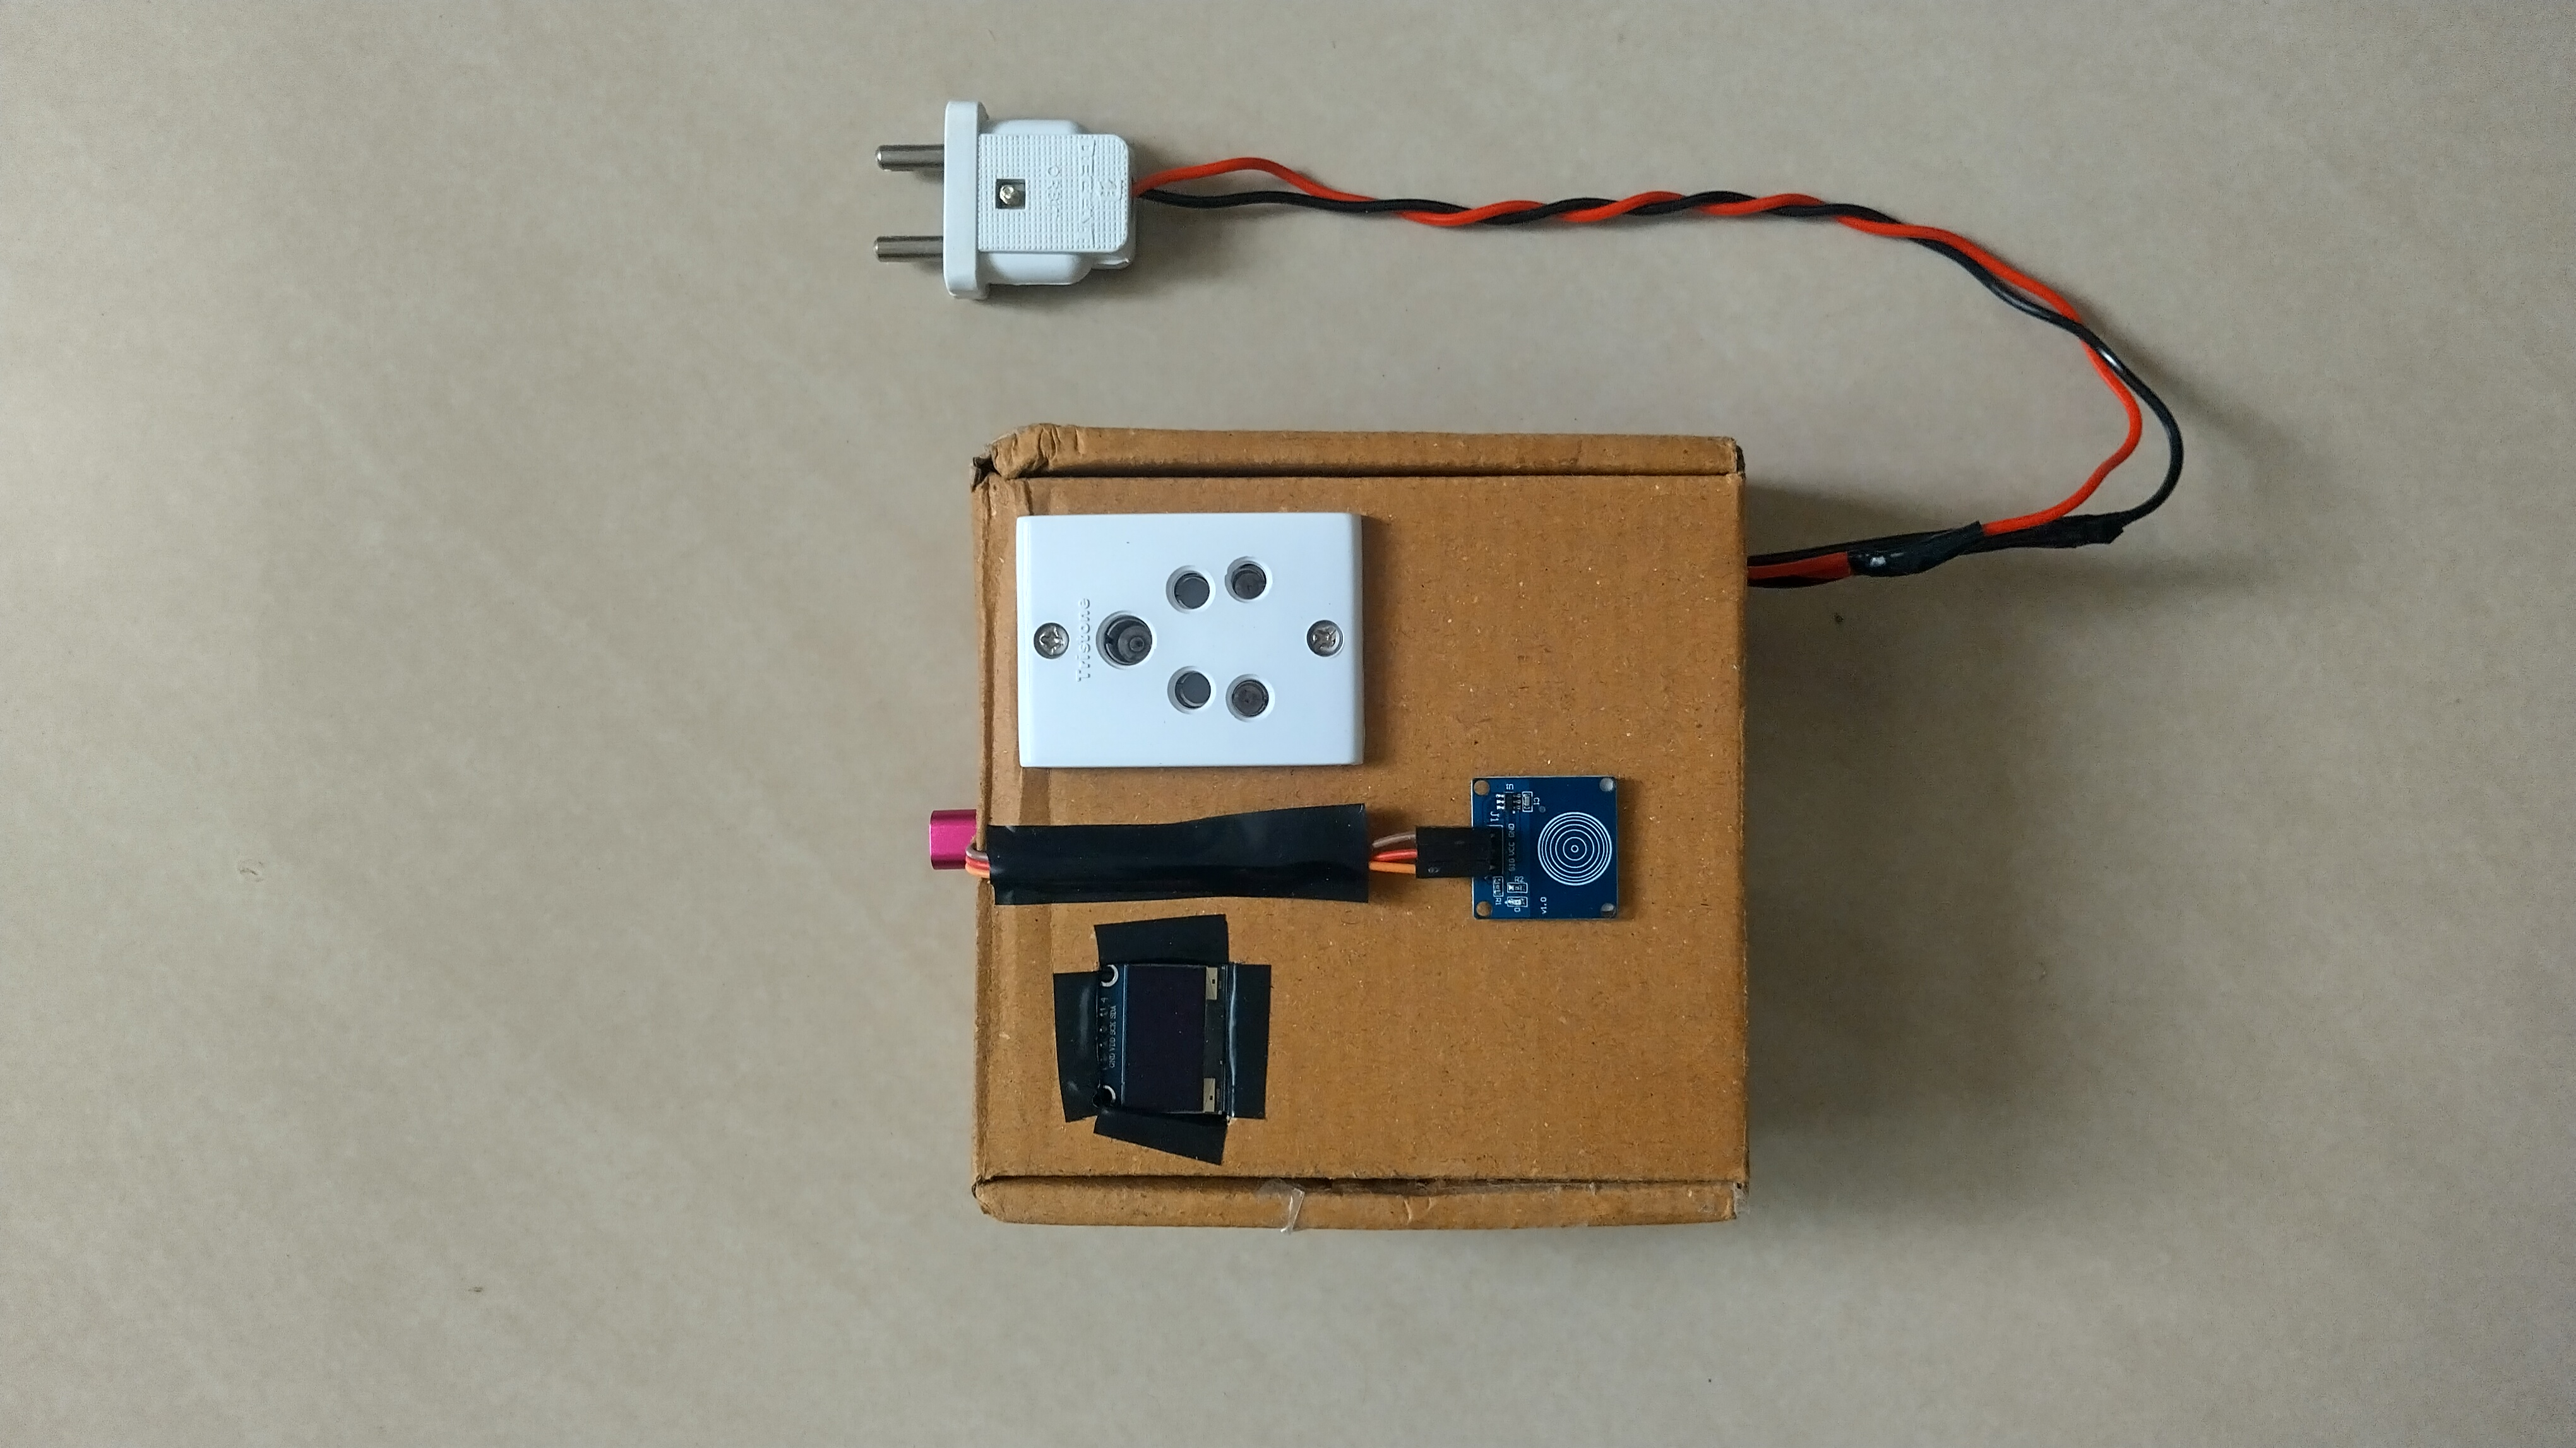
\includegraphics[width=0.72\textwidth]{device.jpg}
		\caption{Assembled device with OLED display showing live readings}
		\label{fig:device}
	\end{figure}
	
	Figure~\ref{fig:device} shows the assembled meter in operating condition. It confirms physical integration of sensing, control, and display blocks in one compact enclosure-ready layout.
	
	\begin{figure}[H]
		\centering
		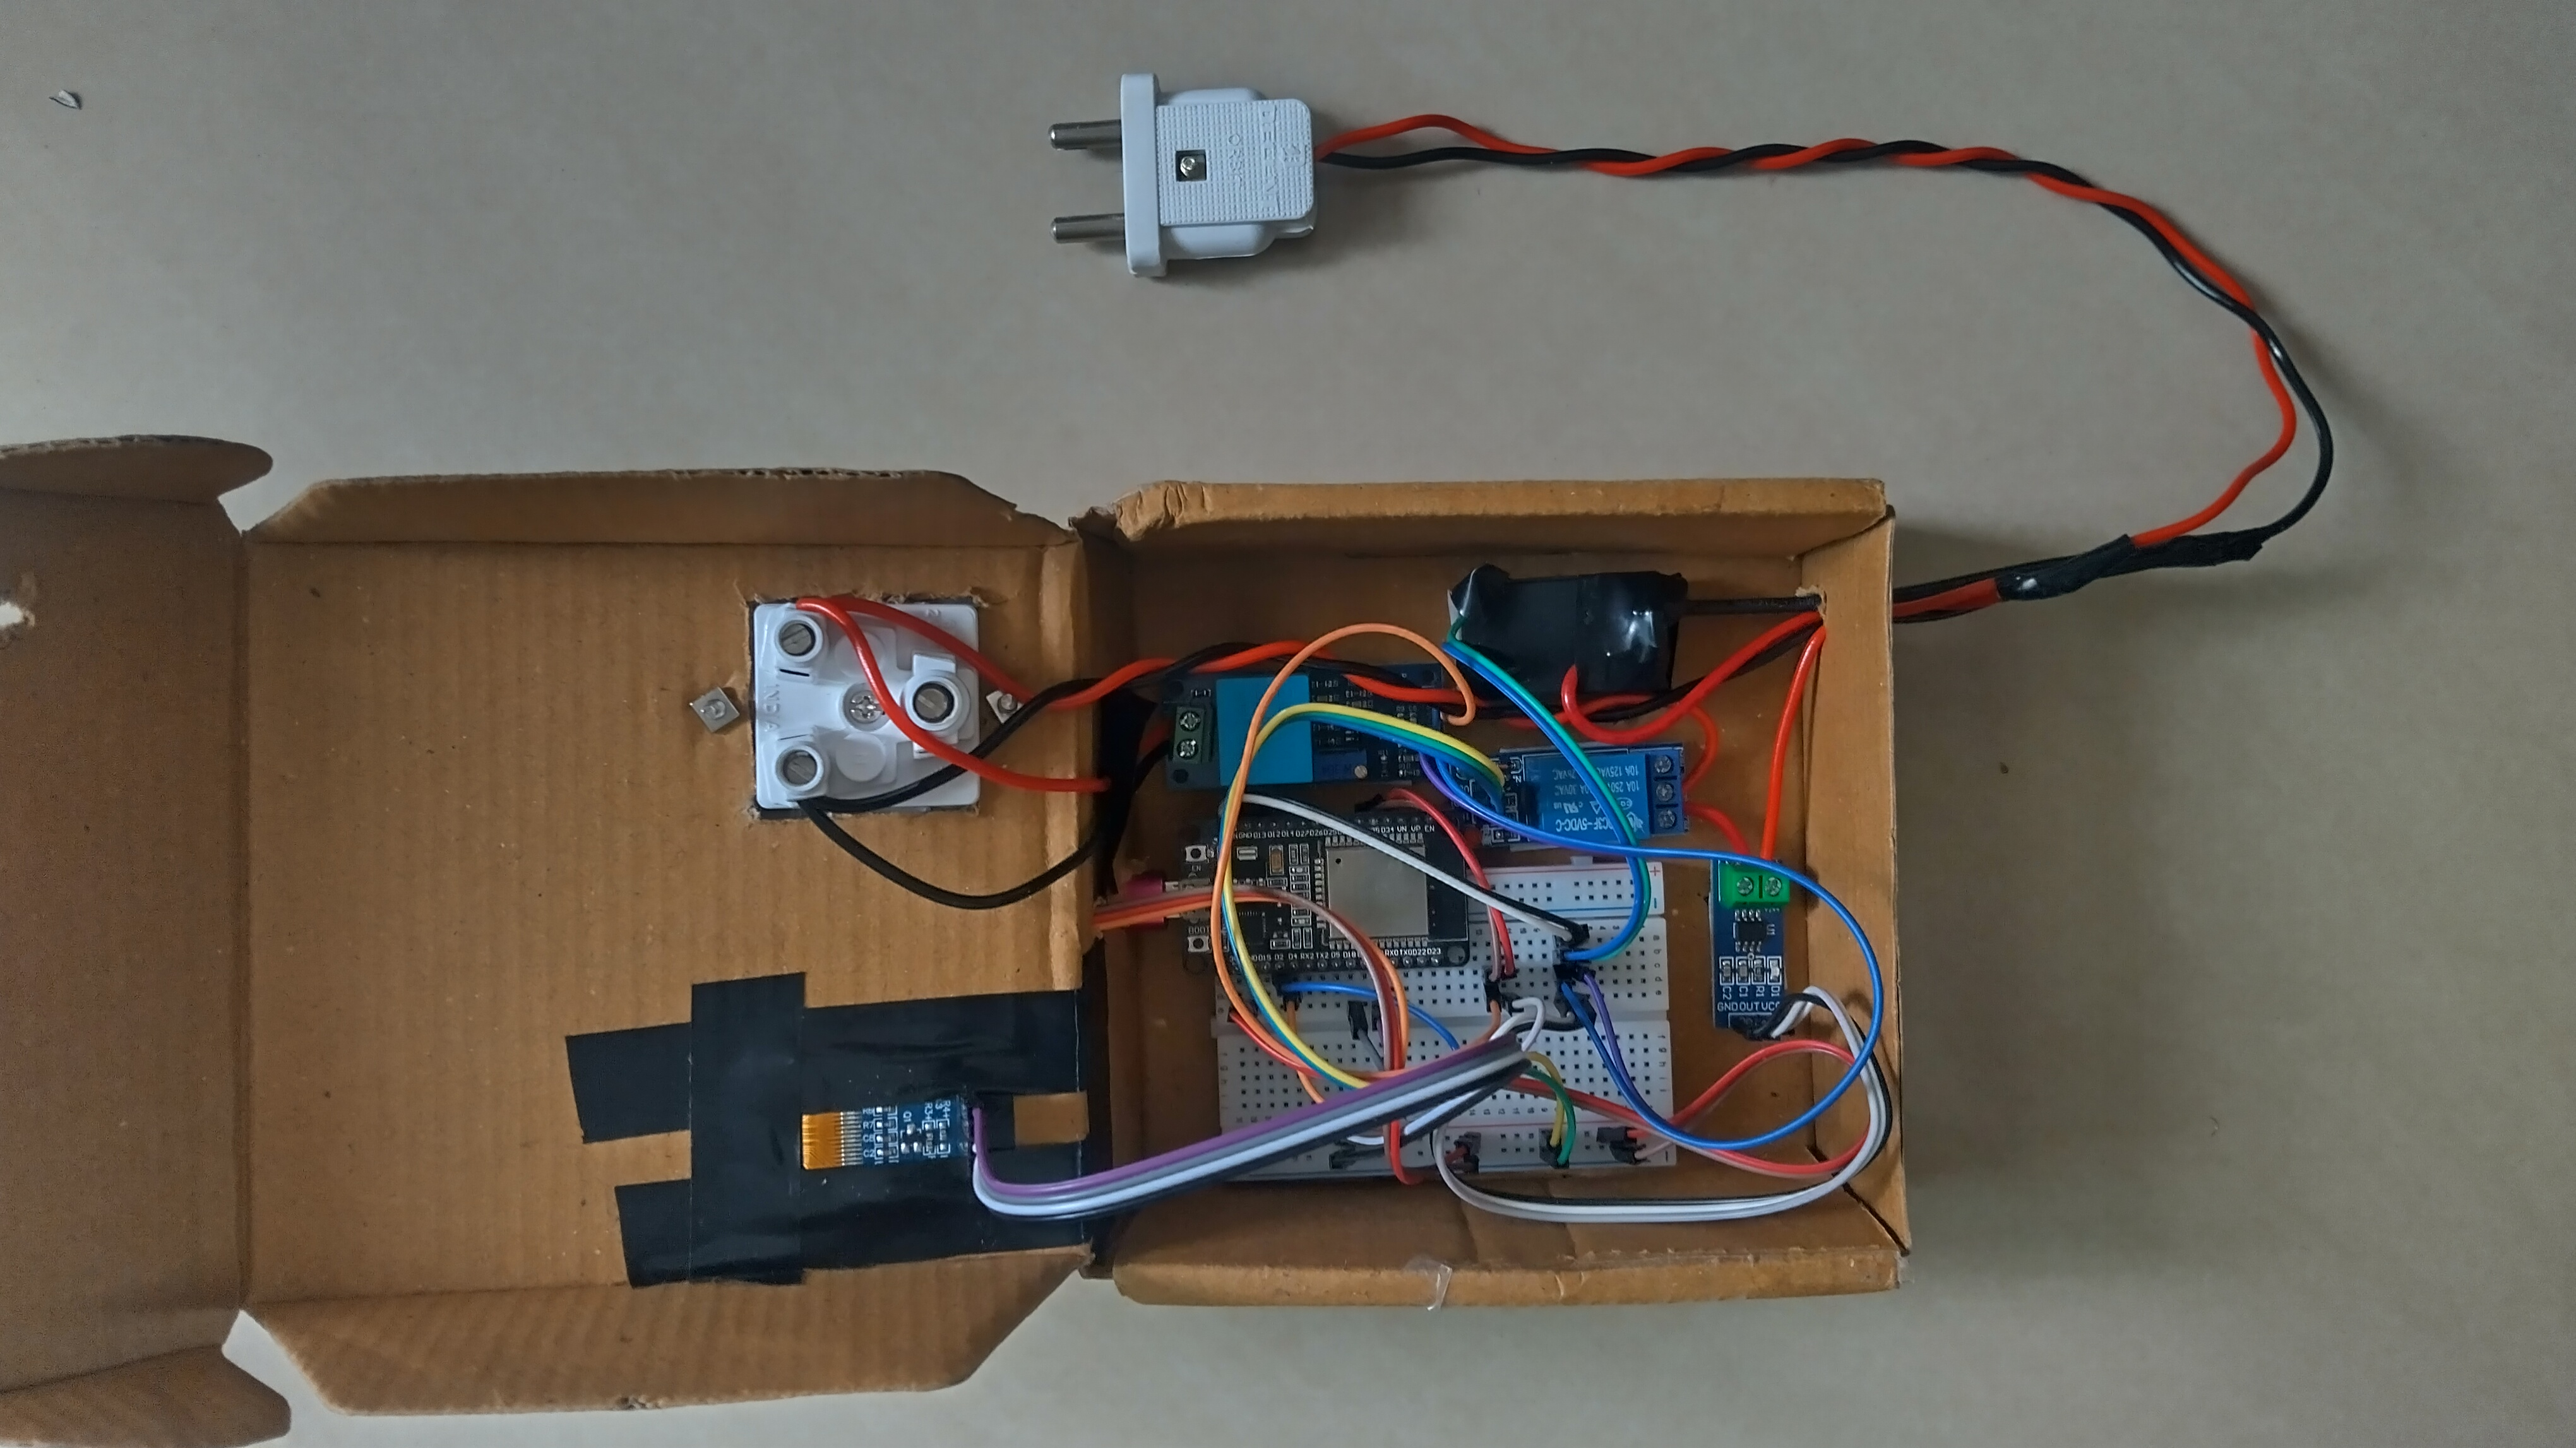
\includegraphics[width=0.72\textwidth]{open-box.jpg}
		\caption{Internal wiring and component layout}
		\label{fig:openbox}
	\end{figure}
	
	Figure~\ref{fig:openbox} shows internal routing and mounting. The layout separates low-voltage control lines from higher-voltage paths to improve reliability and reduce measurement noise pickup.
	
	\subsection{Testing with Appliances}
	
	We tested the system with an electric kettle (600W rated power). Fig.~\ref{fig:kettle-test} shows the kettle connected to the Smart Energy Meter during testing.
	
	\begin{figure}[H]
		\centering
		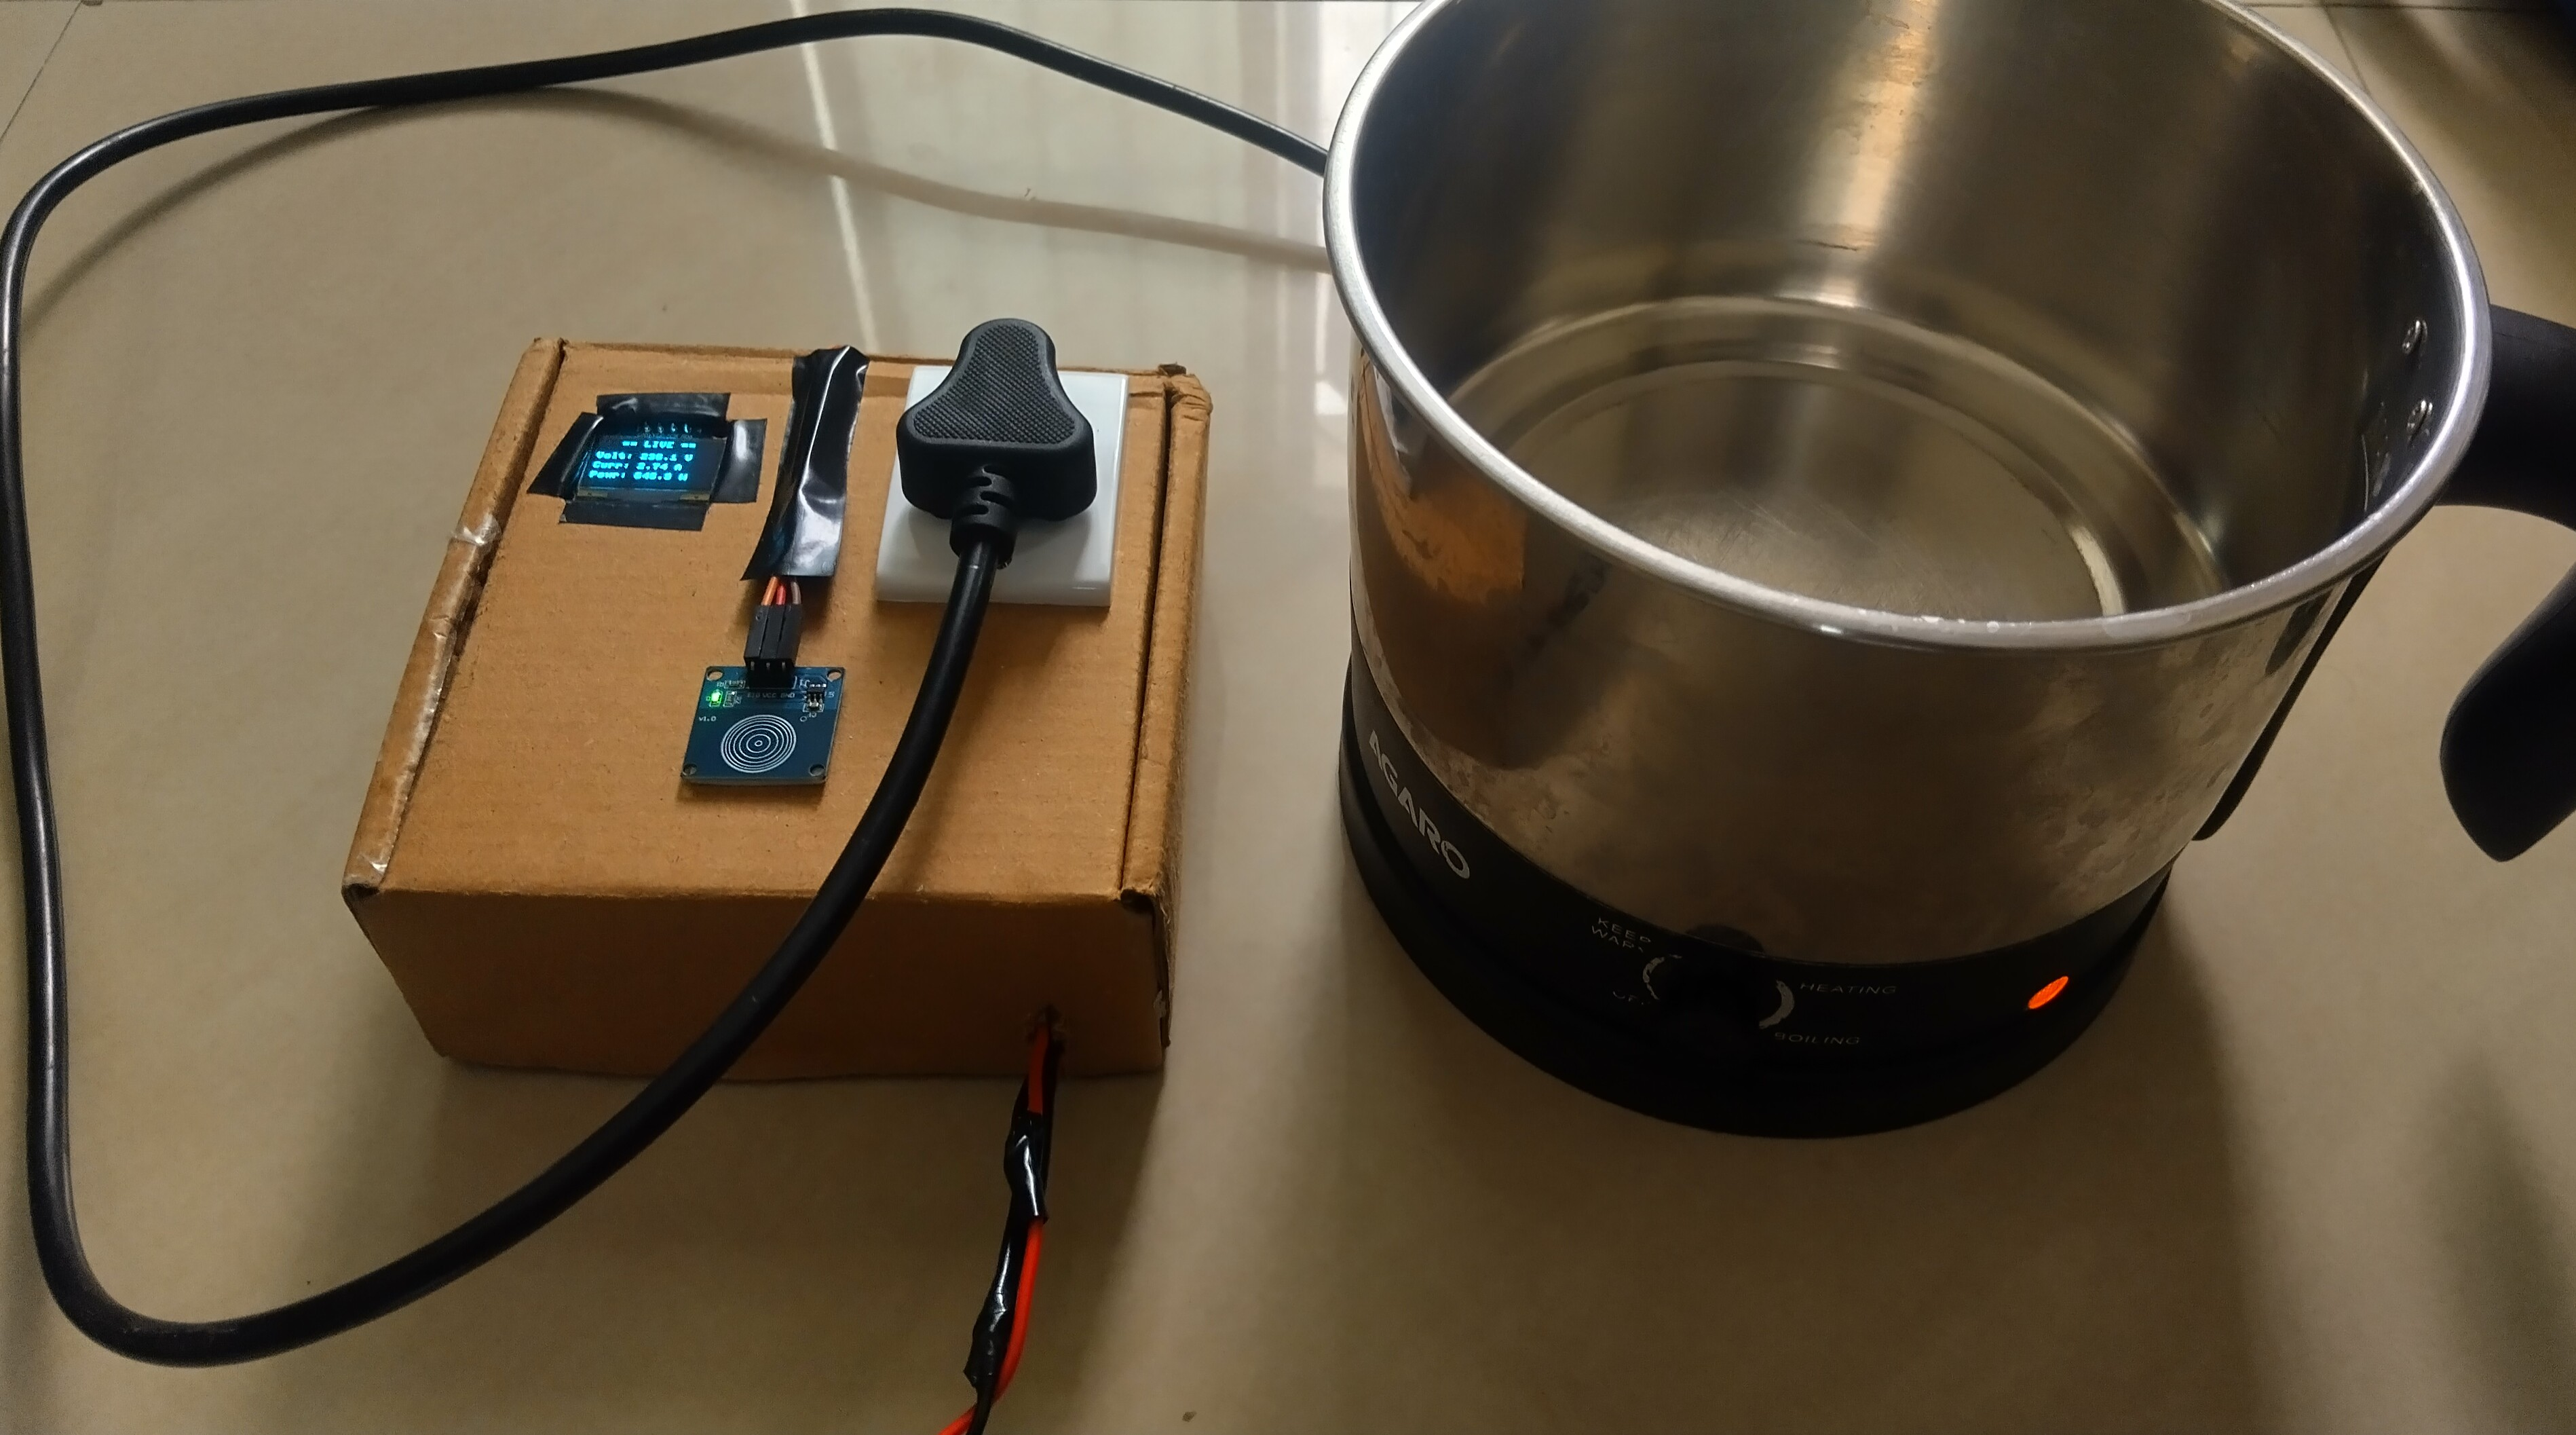
\includegraphics[width=0.72\textwidth]{kettle-test.jpg}
		\caption{Testing setup with electric kettle}
		\label{fig:kettle-test}
	\end{figure}
	
	Figure~\ref{fig:kettle-test} documents the high-load test condition used for calibration checks and repeatability runs. The kettle load is stable enough to evaluate measurement error and relay behavior under sustained demand.
	
	\begin{figure}[H]
		\centering
		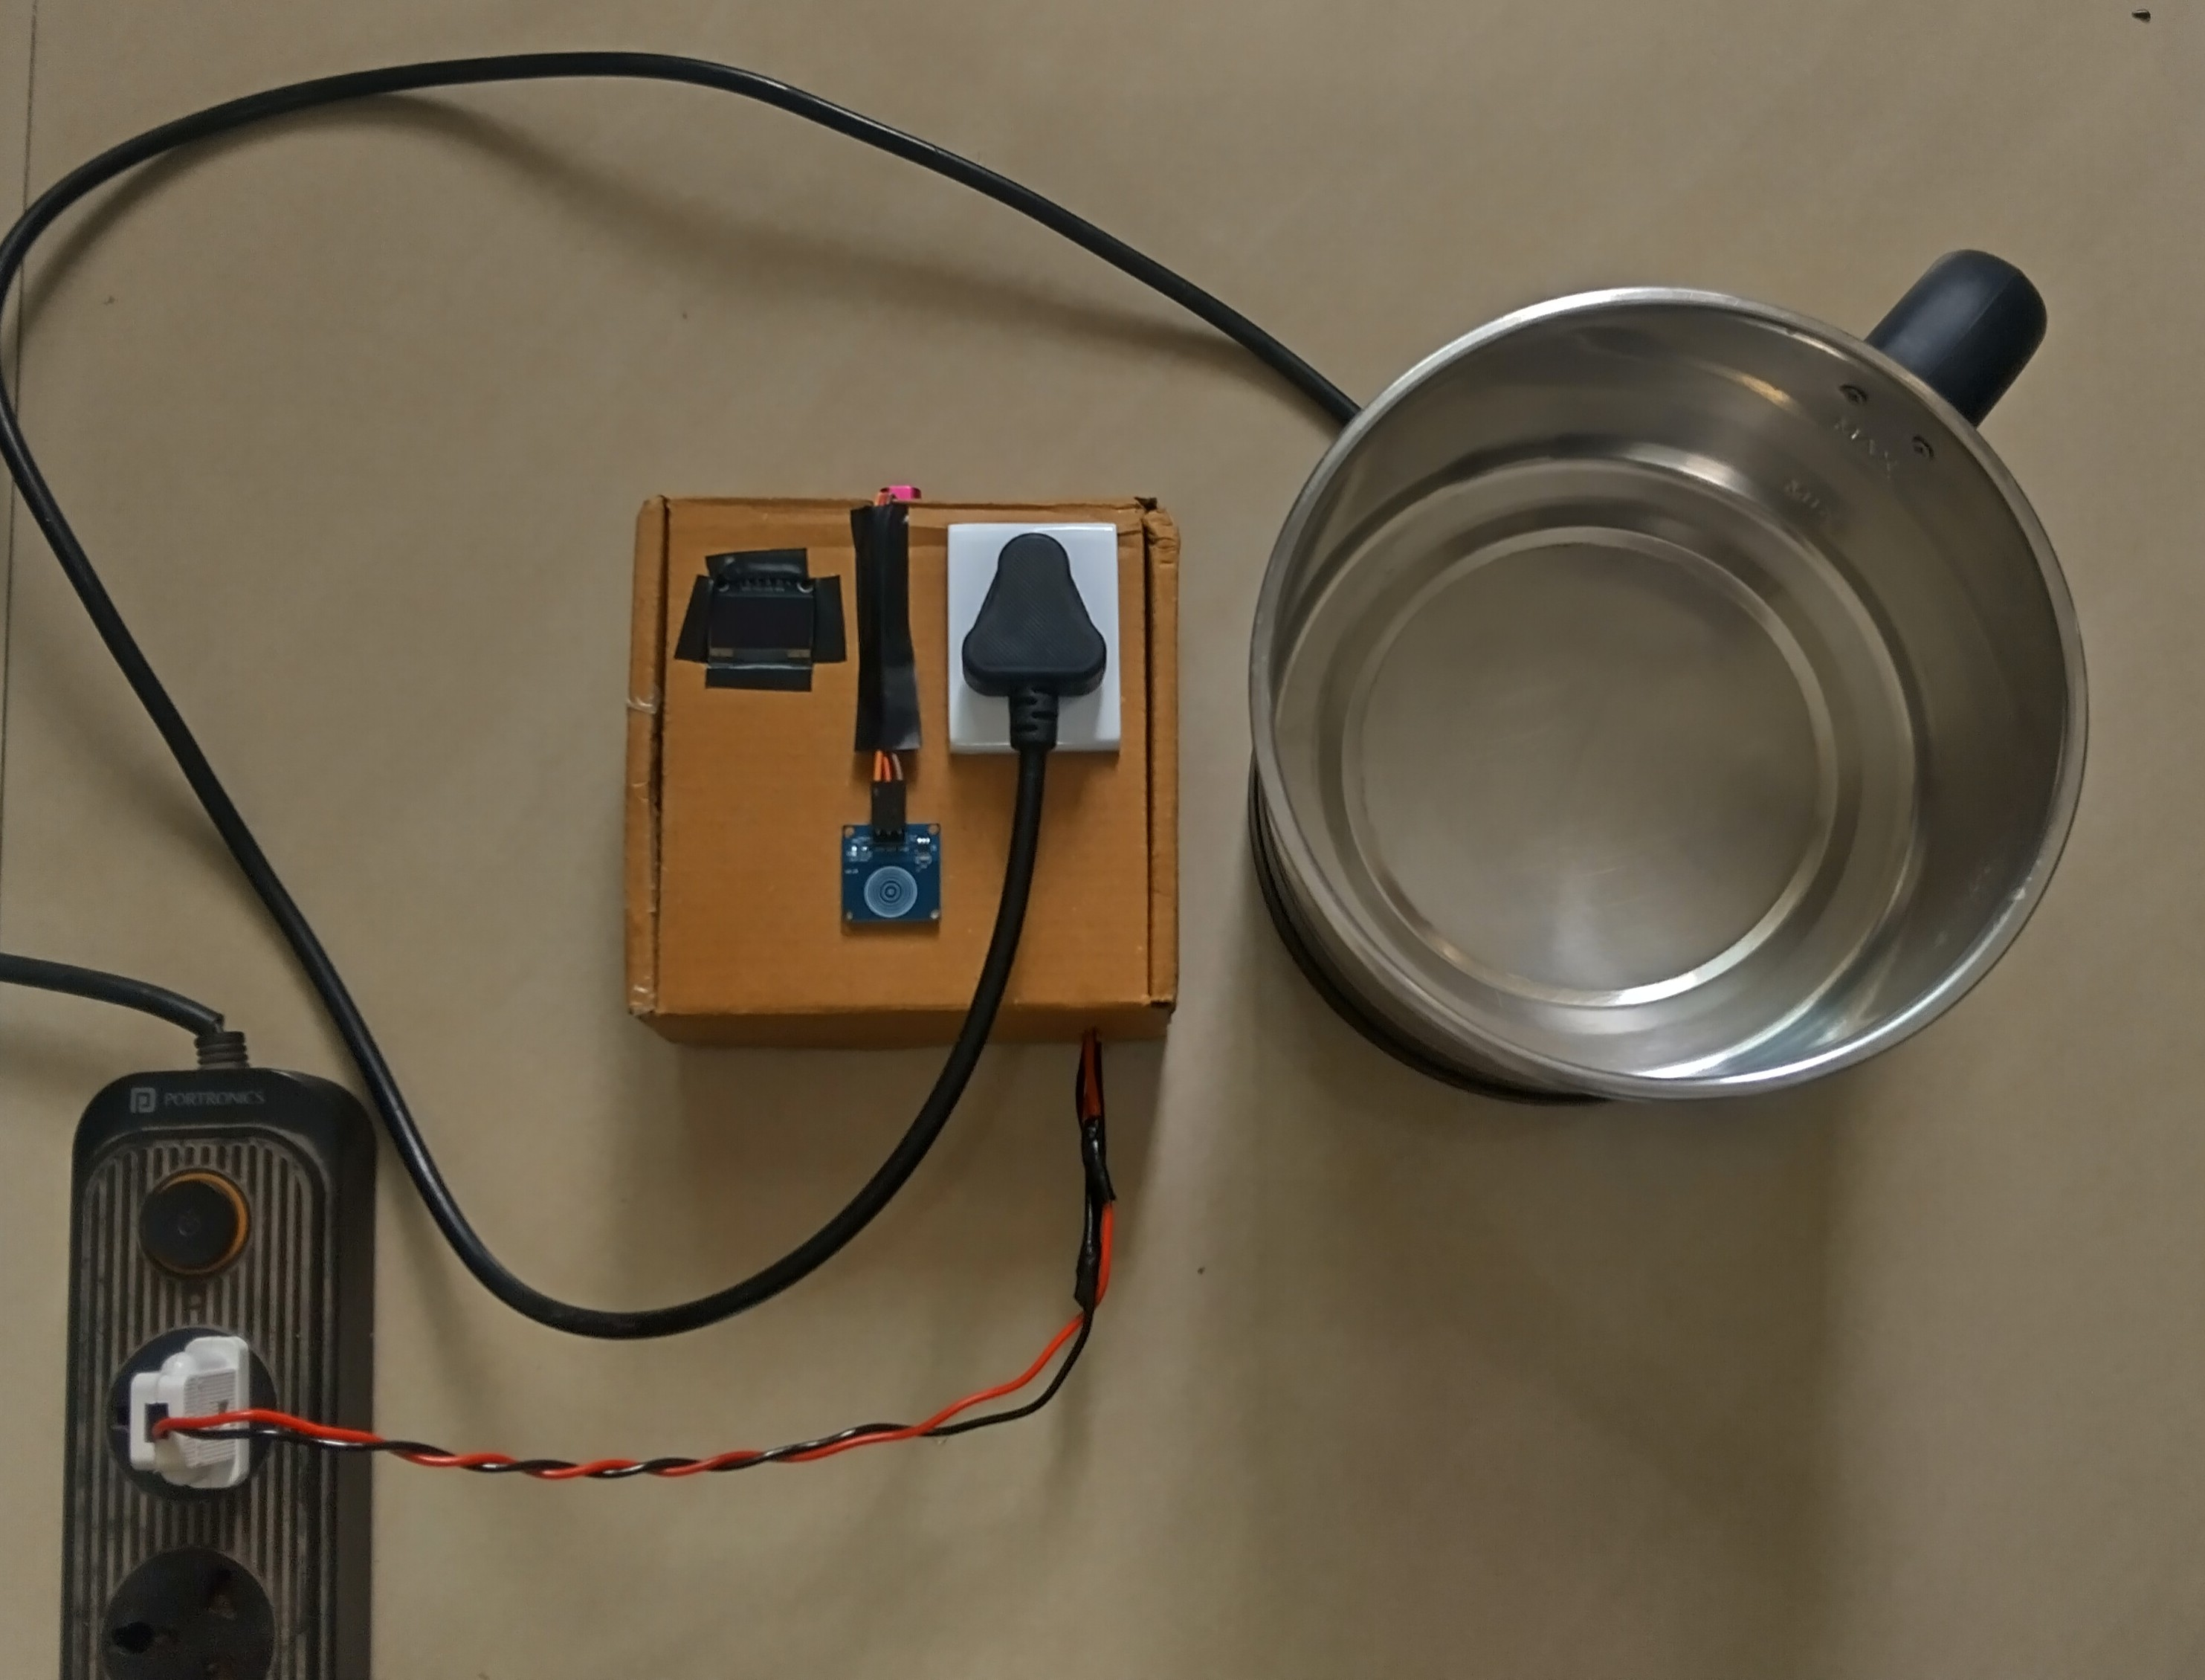
\includegraphics[width=0.72\textwidth]{kettle-tese-2.jpg}
		\caption{Device displaying kettle power consumption}
		\label{fig:kettle-test-2}
	\end{figure}
	
	Figure~\ref{fig:kettle-test-2} captures runtime display output during the same test. The measured values shown on the device are consistent with expected kettle operating range after calibration.
	
	\subsection{Web Dashboard}
	
	The web dashboard provides remote monitoring and control. Fig.~\ref{fig:dashboard} shows the actual dashboard interface.
	
	\begin{figure}[H]
		\centering
		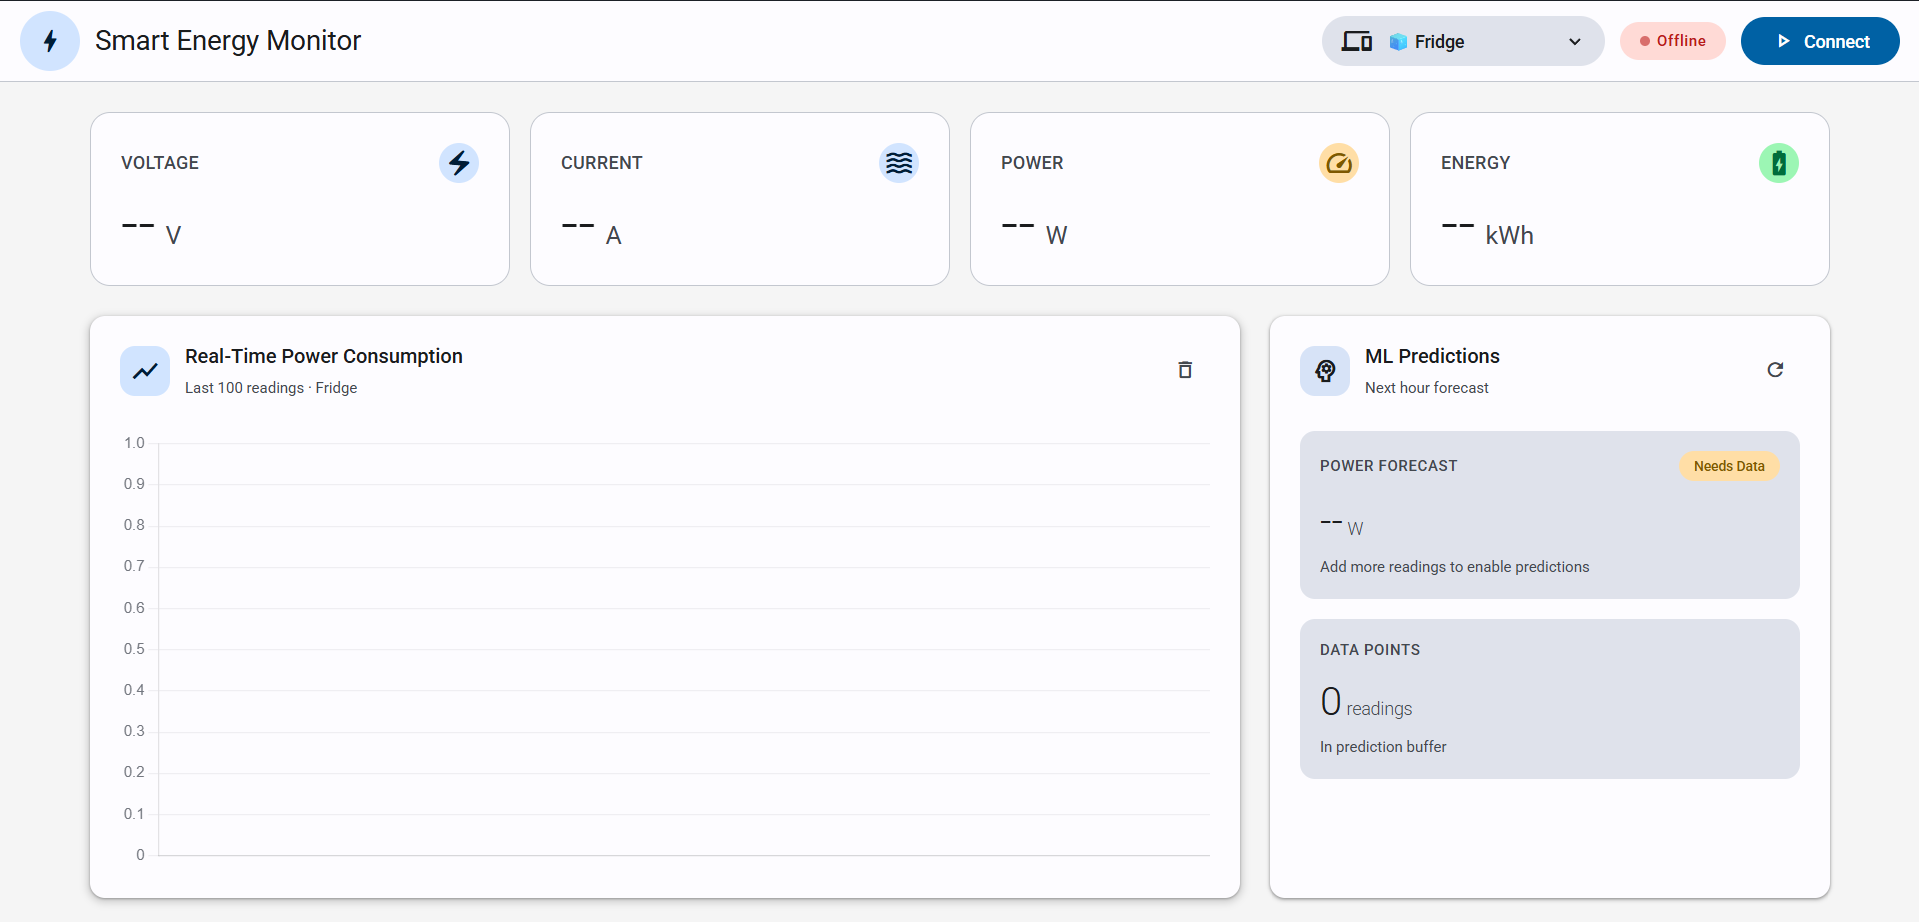
\includegraphics[width=0.78\textwidth]{dashboard.png}
		\caption{Web dashboard showing live power readings and controls}
		\label{fig:dashboard}
	\end{figure}
	
	Figure~\ref{fig:dashboard} presents the live monitoring interface used by end users. It combines key metrics and control actions in one view so operators can react without switching between multiple pages.
	
	\begin{figure}[H]
		\centering
		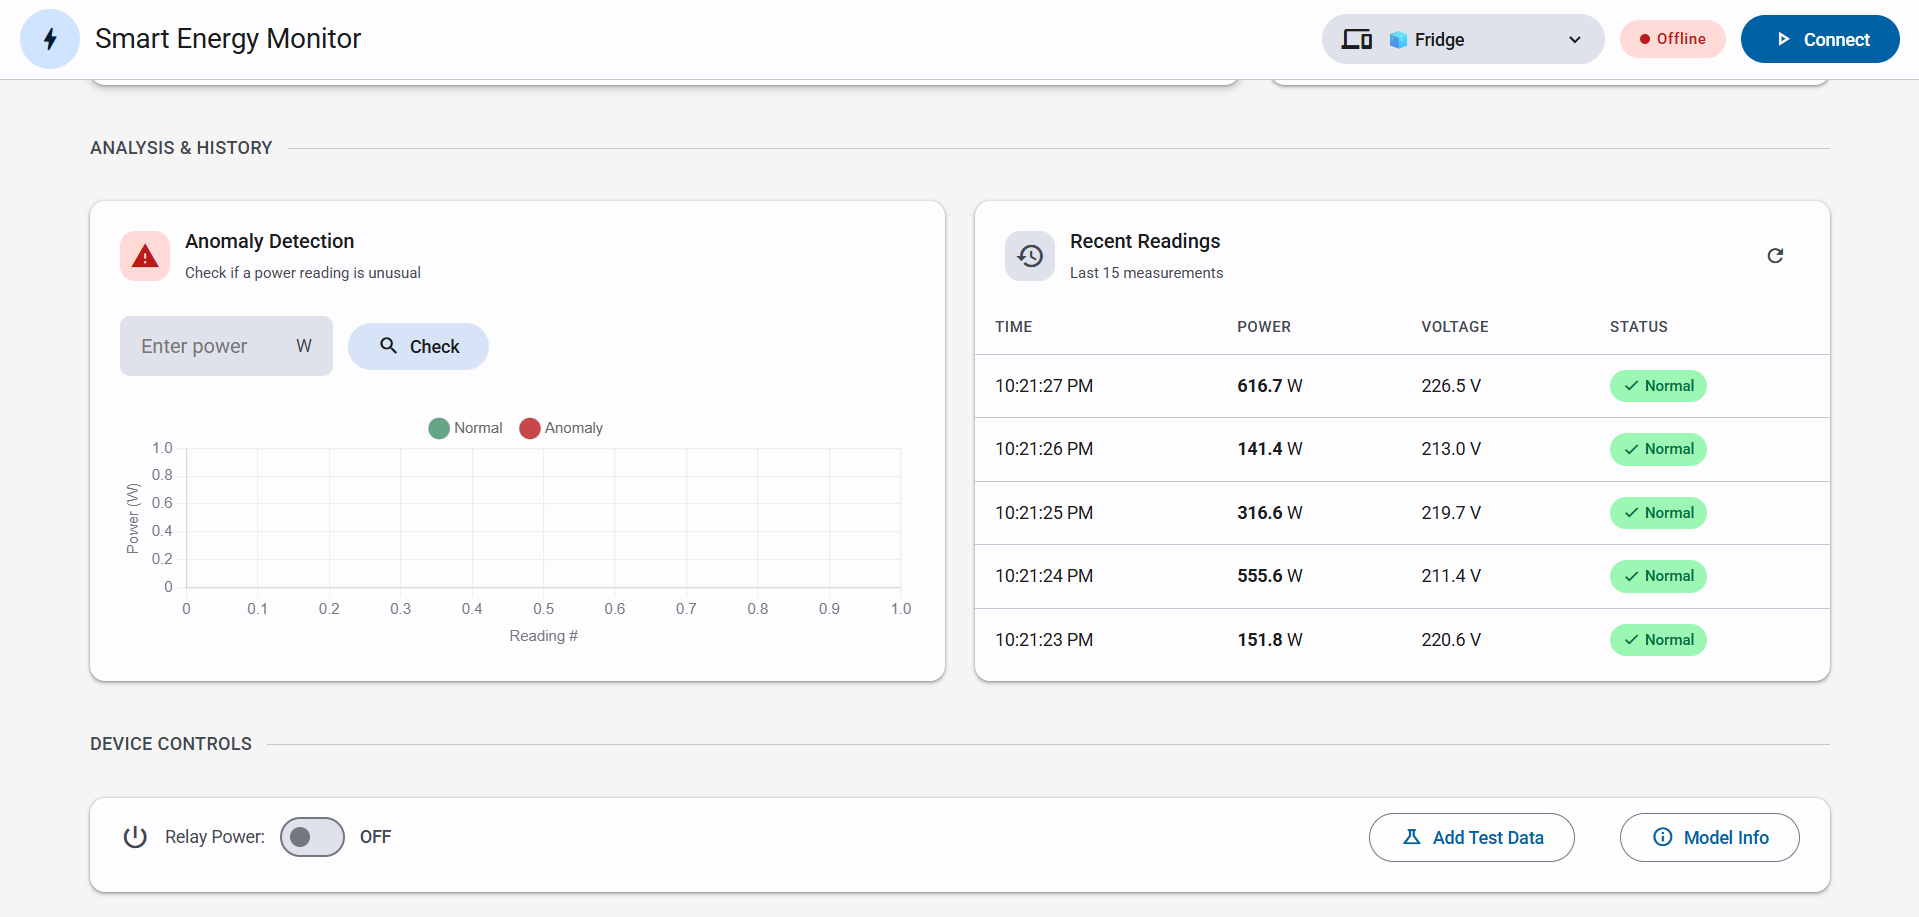
\includegraphics[width=0.78\textwidth]{analysis-history.png}
		\caption{Historical analysis and power consumption graph}
		\label{fig:analysis-history}
	\end{figure}
	
	Figure~\ref{fig:analysis-history} provides trend-level behavior across recent samples. This view helps identify recurring peaks, drift, and deviations that are hard to notice in single live-value readings.
	
	The dashboard includes a live power gauge updated through SSE, direct voltage and current values, a rolling history chart, a relay toggle with visual state, an anomaly alert panel, and a predicted-versus-actual power view for quick diagnosis.
	
	\subsection{OLED Display Screens}
	
	The device has four display screens that cycle when the user long-presses the touch sensor. Table~\ref{tab:oled-screens} describes each screen.
	
	\begin{table}[H]
		\centering
		\caption{OLED display screens}
		\label{tab:oled-screens}
		\vspace{6pt}
		\begin{tabular}{|l|p{8cm}|}
			\hline
			\textbf{Screen} & \textbf{Content} \\
			\hline
			Live & Current voltage (V), current (A), and instantaneous power (W) \\
			\hline
			Energy & Accumulated energy consumption (kWh) and relay state (ON/OFF) \\
			\hline
			Control & Relay state indicator with touch instructions for toggling \\
			\hline
			Debug & Raw calibration values, ADC readings, WiFi status, error count \\
			\hline
		\end{tabular}
	\end{table}
	
	Fig.~\ref{fig:oled-screens-photo} shows captured OLED screens during startup and regular operation.
	
	\begin{figure}[H]
		\centering
		\begin{subfigure}[b]{0.23\textwidth}
			\centering
			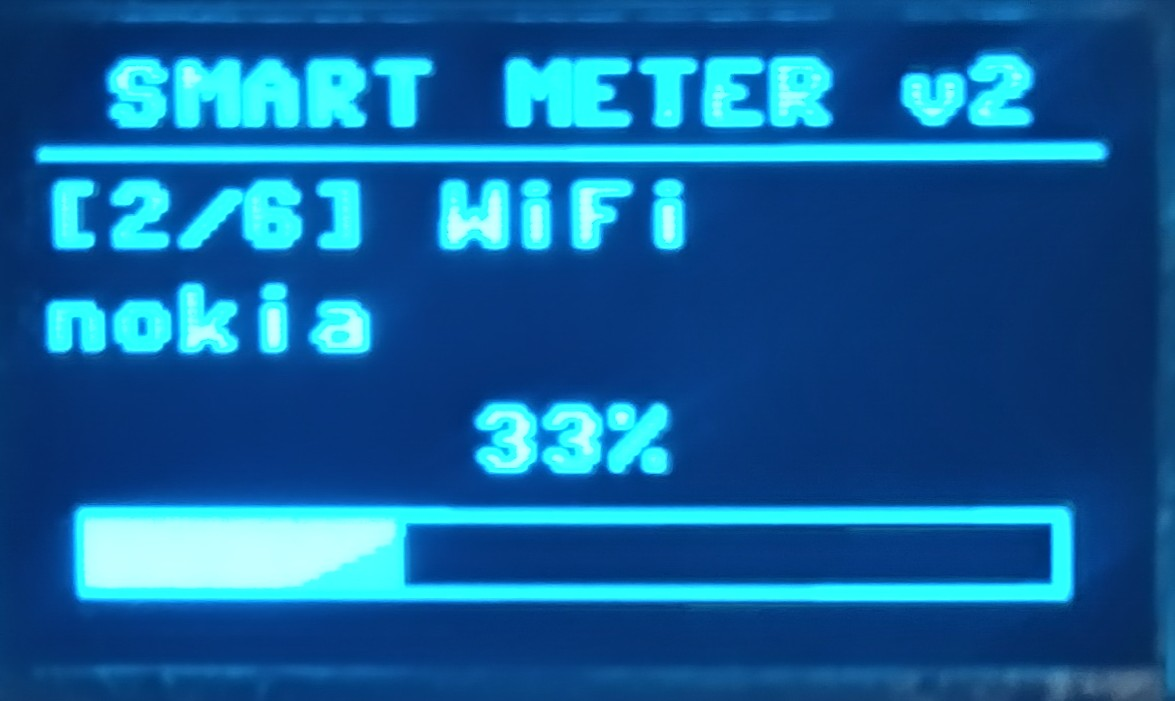
\includegraphics[width=\textwidth]{oled_bootup_1.jpg}
			\caption{Boot 1}
		\end{subfigure}
		\hfill
		\begin{subfigure}[b]{0.23\textwidth}
			\centering
			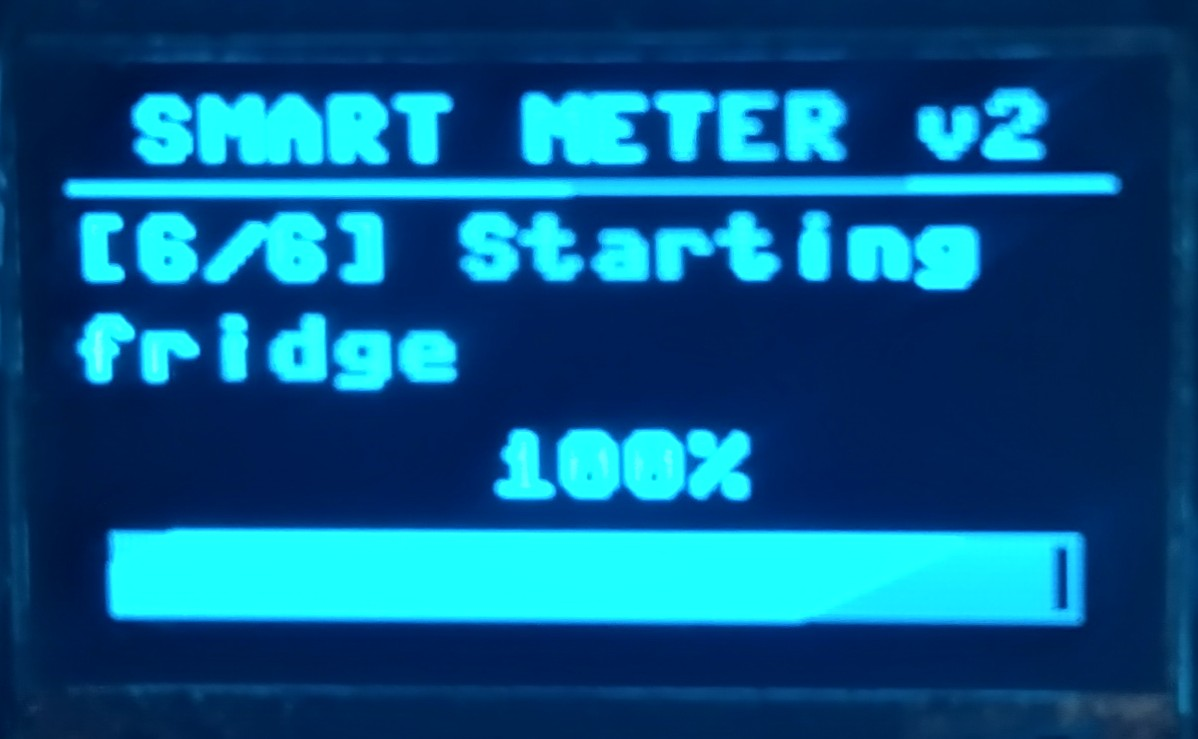
\includegraphics[width=\textwidth]{oled_bootup_2.jpg}
			\caption{Boot 2}
		\end{subfigure}
		\hfill
		\begin{subfigure}[b]{0.23\textwidth}
			\centering
			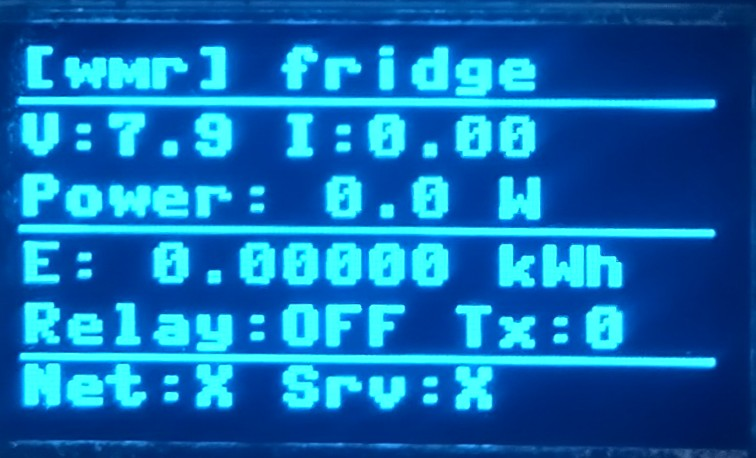
\includegraphics[width=\textwidth]{oled_screen_1.jpg}
			\caption{Live}
		\end{subfigure}
		\hfill
		\begin{subfigure}[b]{0.23\textwidth}
			\centering
			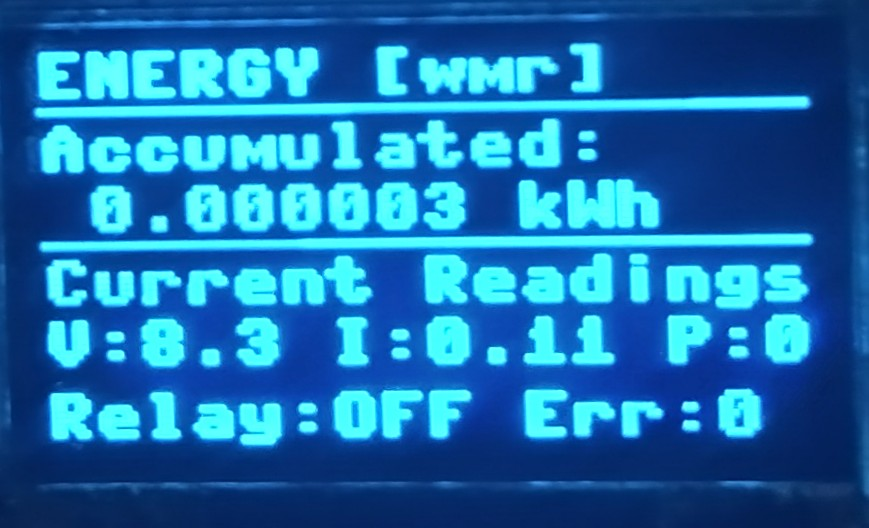
\includegraphics[width=\textwidth]{oled_screen_2.jpg}
			\caption{Energy}
		\end{subfigure}
		
		\vspace{0.2cm}
		
		\begin{subfigure}[b]{0.23\textwidth}
			\centering
			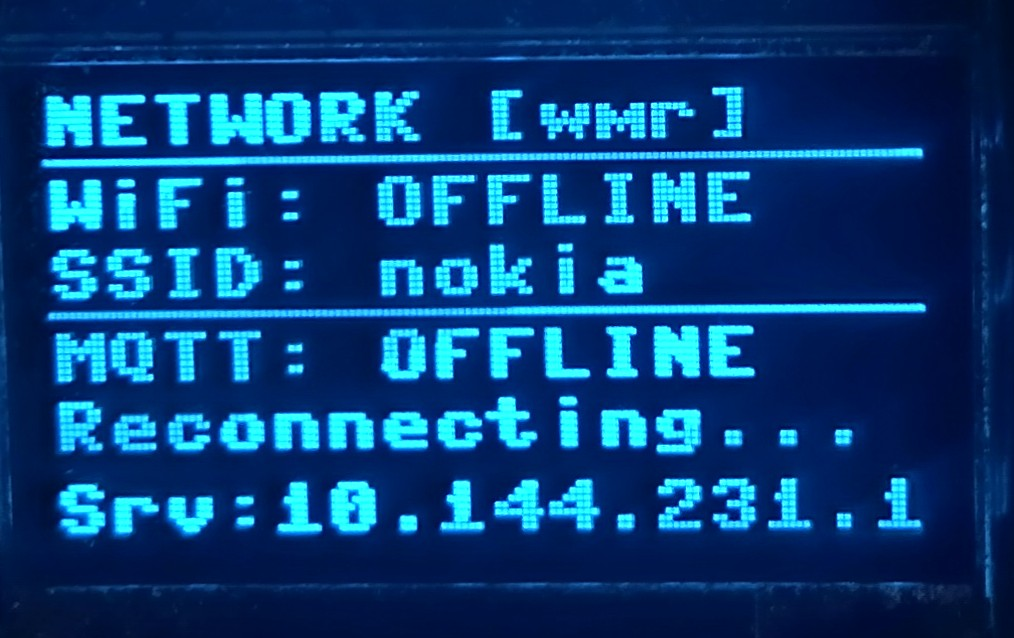
\includegraphics[width=\textwidth]{oled_screen_3.jpg}
			\caption{Control}
		\end{subfigure}
		\hfill
		\begin{subfigure}[b]{0.23\textwidth}
			\centering
			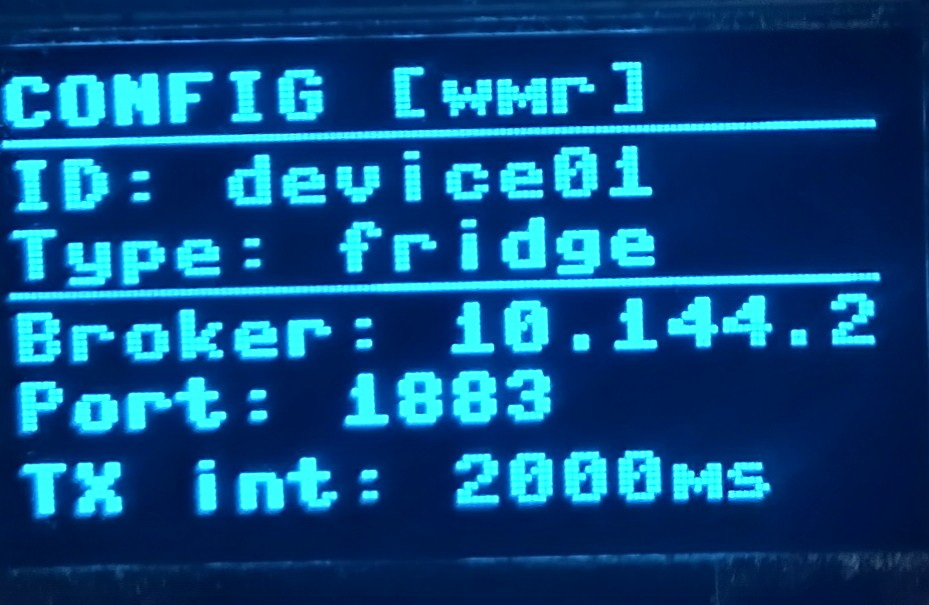
\includegraphics[width=\textwidth]{oled_screen_4.jpg}
			\caption{Debug}
		\end{subfigure}
		\hfill
		\begin{subfigure}[b]{0.23\textwidth}
			\centering
			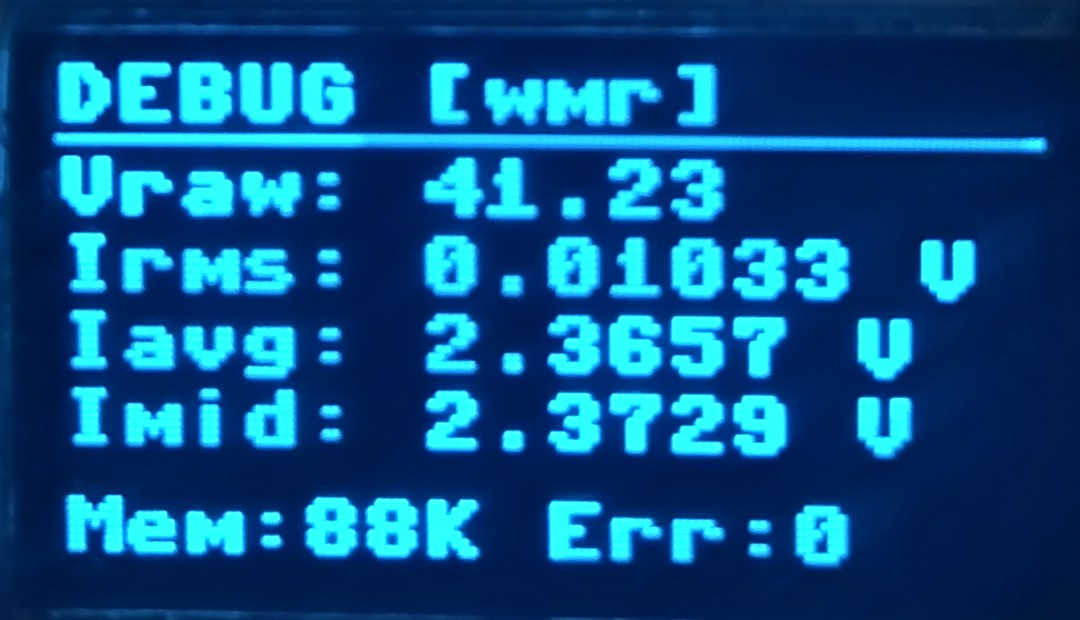
\includegraphics[width=\textwidth]{oled_screen_5.jpg}
			\caption{Runtime}
		\end{subfigure}
		\caption{Captured OLED display screens during boot and runtime}
		\label{fig:oled-screens-photo}
	\end{figure}
	
	Figure~\ref{fig:oled-screens-photo} captures the OLED user journey from boot to runtime pages. These screens provide a local fallback for operation and diagnostics even when the dashboard is not reachable.
	
	A short tap (50--600ms) toggles relay state, and a long press (greater than 600ms) switches to the next screen.
	
	\subsection{ML Model Performance}
	
	Table~\ref{tab:ml} shows the performance metrics for the trained ML models. These metrics were measured on the test set (20\% of data, time-ordered split).
	
	\begin{table}[H]
		\centering
		\caption{ML model performance on test set}
		\label{tab:ml}
		\vspace{6pt}
		\begin{tabular}{|l|l|r|p{5cm}|}
			\hline
			\textbf{Model} & \textbf{Metric} & \textbf{Value} & \textbf{Interpretation} \\
			\hline
			Power predictor & MAE & 42.3 W & Average error in power prediction \\
			\hline
			Power predictor & R\textsuperscript{2} & 0.87 & Model explains 87\% of variance \\
			\hline
			On/off classifier & Accuracy & 94\% & Correctly classifies device state \\
			\hline
			Anomaly detector & Precision & 89\% & 89\% of flagged anomalies are real \\
			\hline
		\end{tabular}
	\end{table}
	
	\begin{table}[H]
		\centering
		\caption{Appliance-wise model snapshot from processed PLEGMA data}
		\label{tab:appliance-ml}
		\vspace{6pt}
		\small
		\setlength{\tabcolsep}{4pt}
		\begin{tabularx}{\textwidth}{|p{2.1cm}|p{1.9cm}|p{1.6cm}|p{2.2cm}|X|}
			\hline
			\textbf{Appliance} & \textbf{Regression R\textsuperscript{2}} & \textbf{MAE (W)} & \textbf{Classifier Accuracy} & \textbf{Anomaly rate} \\
			\hline
			AC 1 & 0.876 & 85.2 & 0.923 & 2.1\% \\
			\hline
			AC 2 & 0.842 & 92.1 & 0.908 & 2.0\% \\
			\hline
			Boiler & 0.723 & 156.3 & 0.956 & 2.3\% \\
			\hline
			Fridge & 0.912 & 8.4 & 0.978 & 1.8\% \\
			\hline
			Washing machine & 0.654 & 45.6 & 0.887 & 2.0\% \\
			\hline
		\end{tabularx}
		\setlength{\tabcolsep}{6pt}
		\normalsize
	\end{table}
	
	Table~\ref{tab:appliance-ml} shows that continuously cycling appliances such as fridge are easier to model than bursty appliances such as washing machines. This behavior matches practical usage patterns and supports the decision to maintain appliance-specific models instead of a single global predictor.
	
	\subsection{Sample Telemetry Data}
	
	A typical telemetry JSON payload transmitted from the ESP32 to the backend:
	
	\begin{lstlisting}[basicstyle=\ttfamily\small, frame=single]
	{
	  "voltage": 228.5,
	  "current": 2.34,
	  "power": 534.7,
	  "energy": 1.234,
	  "relay": true,
	  "timestamp": "2025-04-07T10:30:00"
	}
	\end{lstlisting}
	
	The backend parses this JSON, runs ML inference, stores the data in CSV format, and broadcasts updates to connected dashboards.
	
	\subsection{Measurement Accuracy}
	
	We tested the system against a commercial power meter (calibrated to $\pm$0.5\% accuracy) using two appliances: an electric kettle (600W resistive load) and a laptop charger (65W switching supply).
	
	Table~\ref{tab:accuracy} shows the measurement accuracy after calibration.
	
	\begin{table}[H]
		\centering
		\caption{Measurement accuracy results}
		\label{tab:accuracy}
		\vspace{6pt}
		\begin{tabular}{|l|c|c|}
			\hline
			\textbf{Parameter} & \textbf{Kettle (600W)} & \textbf{Charger (65W)} \\
			\hline
			Voltage error & $\pm$1.5\% & $\pm$1.5\% \\
			\hline
			Current error & $\pm$2\% & $\pm$5\% \\
			\hline
			Power error & $\pm$2.5\% & $\pm$5\% \\
			\hline
		\end{tabular}
	\end{table}
	
	The ACS712 current sensor is the main source of error. At low currents (below 0.5A), the sensor's 100mV/A resolution becomes a limiting factor. For the laptop charger (approximately 0.3A), the current measurement error was higher due to this resolution limitation.
	
	\newpage
	
	\section{Conclusion and Future Work}\label{sec:conclusion}
	
	\subsection{Conclusion}
	
	This project implemented a per-appliance energy monitoring system using the ESP32 DevKit V1 microcontroller. The system addresses a practical limitation of whole-house electricity meters: they show aggregate consumption without revealing which devices use the most power.
	
	\textbf{What we built:} The project delivers a hardware module using off-the-shelf parts (about Rs. 1,500), MicroPython firmware for sensing and MQTT communication, a Flask backend with ML-assisted anomaly detection, and a live web dashboard with relay control.
	
	\textbf{What the ML adds:}
	
	The machine learning component goes beyond simple threshold alerts. The LightGBM power predictor (R\textsuperscript{2} = 0.87) learns usage patterns and can identify when consumption differs from the norm. The Isolation Forest detector catches subtle changes that may indicate equipment degradation. The on/off classifier (94\% accuracy) predicts expected device state.
	
	\textbf{Testing results:}
	
	We tested the system on two appliances: an electric kettle (600W) and a laptop charger (65W). After calibration, the kettle readings matched a reference meter within 2.5\%. The charger readings were within 5\% due to ACS712 sensor limitations at low currents. The relay switches correctly. Dashboard updates arrive in real time via SSE.
	
	\subsection{Future Work}
	
	Several improvements can make this system more practical in real deployments. The first is true power-factor measurement through phase-angle estimation, which improves accuracy for motors and other inductive loads. The second is three-phase support for larger installations. The third is local buffering and delayed sync so data is not lost during WiFi drops. Cost integration with tariff slabs would also make the dashboard easier to use for budgeting decisions.
	
	\newpage
	\label{sec:references}
	\begin{thebibliography}{16}
		\bibitem{plegma}
		S. Athanasoulias \emph{et al.}, ``The Plegma dataset: Domestic appliance-level and aggregate electricity demand with metadata from Greece,'' \emph{Scientific Data}, vol. 11, p. 376, 2024, doi: 10.1038/s41597-024-03208-0.
		
		\bibitem{smartmeter-analytics}
		Y. Wang, Q. Chen, T. Hong, and C. Kang, ``Review of smart meter data analytics: Applications, methodologies, and challenges,'' \emph{IEEE Transactions on Smart Grid}, vol. 10, no. 3, pp. 3125--3148, 2019.
		
		\bibitem{feedback}
		A. Faruqui, D. Sergici, and A. Sharif, ``The impact of informational feedback on energy consumption: A survey of the experimental evidence,'' \emph{Energy}, vol. 35, no. 4, pp. 1598--1608, 2010.
		
		\bibitem{ampds}
		S. Makonin, F. Popowich, L. Bartram, B. Gill, and I. V. Bajic, ``AMPds: A public dataset for load disaggregation and eco-feedback research,'' in \emph{Proc. IEEE Electrical Power and Energy Conference (EPEC)}, 2013.
		
		\bibitem{iforest}
		F. T. Liu, K. M. Ting, and Z.-H. Zhou, ``Isolation forest,'' in \emph{Proc. IEEE International Conference on Data Mining (ICDM)}, 2008, pp. 413--422.
		
		\bibitem{lightgbm}
		G. Ke \emph{et al.}, ``LightGBM: A highly efficient gradient boosting decision tree,'' in \emph{Advances in Neural Information Processing Systems}, vol. 30, 2017.
		
		\bibitem{sklearn}
		F. Pedregosa \emph{et al.}, ``Scikit-learn: Machine learning in Python,'' \emph{Journal of Machine Learning Research}, vol. 12, pp. 2825--2830, 2011.
		
		\bibitem{mqtt}
		OASIS Standard, \emph{MQTT Version 5.0}, 2019. [Online]. Available: \url{https://docs.oasis-open.org/mqtt/mqtt/v5.0/mqtt-v5.0.html}
		
		\bibitem{esp32-trm}
		Espressif Systems, \emph{ESP32 Technical Reference Manual}, 2023. [Online]. Available: \url{https://www.espressif.com/sites/default/files/documentation/esp32_technical_reference_manual_en.pdf}
		
		\bibitem{micropython-esp32}
		MicroPython Documentation, ``Quick reference for the ESP32,'' 2024. [Online]. Available: \url{https://docs.micropython.org/en/latest/esp32/quickref.html}
		
		\bibitem{flask}
		Pallets Projects, ``Flask documentation,'' 2024. [Online]. Available: \url{https://flask.palletsprojects.com/}
		
		\bibitem{nanomq}
		EMQ Technologies, ``NanoMQ: Ultra-lightweight MQTT broker,'' 2024. [Online]. Available: \url{https://nanomq.io/}
		
		\bibitem{chartjs}
		Chart.js Contributors, ``Chart.js documentation,'' 2024. [Online]. Available: \url{https://www.chartjs.org/docs/latest/}
		
		\bibitem{acs712}
		Allegro MicroSystems, \emph{ACS712 Fully Integrated, Hall-Effect-Based Linear Current Sensor}, Datasheet, 2020.
		
		\bibitem{hlkpm01}
		Hi-Link Electronic, \emph{HLK-PM01 AC-DC Power Module}, Datasheet, 2019.
		
		\bibitem{ssd1306}
		Solomon Systech, \emph{SSD1306 128x64 Dot Matrix OLED/PLED Segment/Common Driver with Controller}, Datasheet, 2008.
	\end{thebibliography}
	
\end{document}
